\documentclass[twoside]{book}

% Packages required by doxygen
\usepackage{fixltx2e}
\usepackage{calc}
\usepackage{doxygen}
\usepackage[export]{adjustbox} % also loads graphicx
\usepackage{graphicx}
\usepackage[utf8]{inputenc}
\usepackage{makeidx}
\usepackage{multicol}
\usepackage{multirow}
\PassOptionsToPackage{warn}{textcomp}
\usepackage{textcomp}
\usepackage[nointegrals]{wasysym}
\usepackage[table]{xcolor}

% Font selection
\usepackage[T1]{fontenc}
\usepackage[scaled=.90]{helvet}
\usepackage{courier}
\usepackage{amssymb}
\usepackage{sectsty}
\renewcommand{\familydefault}{\sfdefault}
\allsectionsfont{%
  \fontseries{bc}\selectfont%
  \color{darkgray}%
}
\renewcommand{\DoxyLabelFont}{%
  \fontseries{bc}\selectfont%
  \color{darkgray}%
}
\newcommand{\+}{\discretionary{\mbox{\scriptsize$\hookleftarrow$}}{}{}}

% Page & text layout
\usepackage{geometry}
\geometry{%
  a4paper,%
  top=2.5cm,%
  bottom=2.5cm,%
  left=2.5cm,%
  right=2.5cm%
}
\tolerance=750
\hfuzz=15pt
\hbadness=750
\setlength{\emergencystretch}{15pt}
\setlength{\parindent}{0cm}
\setlength{\parskip}{3ex plus 2ex minus 2ex}
\makeatletter
\renewcommand{\paragraph}{%
  \@startsection{paragraph}{4}{0ex}{-1.0ex}{1.0ex}{%
    \normalfont\normalsize\bfseries\SS@parafont%
  }%
}
\renewcommand{\subparagraph}{%
  \@startsection{subparagraph}{5}{0ex}{-1.0ex}{1.0ex}{%
    \normalfont\normalsize\bfseries\SS@subparafont%
  }%
}
\makeatother

% Headers & footers
\usepackage{fancyhdr}
\pagestyle{fancyplain}
\fancyhead[LE]{\fancyplain{}{\bfseries\thepage}}
\fancyhead[CE]{\fancyplain{}{}}
\fancyhead[RE]{\fancyplain{}{\bfseries\leftmark}}
\fancyhead[LO]{\fancyplain{}{\bfseries\rightmark}}
\fancyhead[CO]{\fancyplain{}{}}
\fancyhead[RO]{\fancyplain{}{\bfseries\thepage}}
\fancyfoot[LE]{\fancyplain{}{}}
\fancyfoot[CE]{\fancyplain{}{}}
\fancyfoot[RE]{\fancyplain{}{\bfseries\scriptsize Generated by Doxygen }}
\fancyfoot[LO]{\fancyplain{}{\bfseries\scriptsize Generated by Doxygen }}
\fancyfoot[CO]{\fancyplain{}{}}
\fancyfoot[RO]{\fancyplain{}{}}
\renewcommand{\footrulewidth}{0.4pt}
\renewcommand{\chaptermark}[1]{%
  \markboth{#1}{}%
}
\renewcommand{\sectionmark}[1]{%
  \markright{\thesection\ #1}%
}

% Indices & bibliography
\usepackage{natbib}
\usepackage[titles]{tocloft}
\setcounter{tocdepth}{3}
\setcounter{secnumdepth}{5}
\makeindex

% Hyperlinks (required, but should be loaded last)
\usepackage{ifpdf}
\ifpdf
  \usepackage[pdftex,pagebackref=true]{hyperref}
\else
  \usepackage[ps2pdf,pagebackref=true]{hyperref}
\fi
\hypersetup{%
  colorlinks=true,%
  linkcolor=blue,%
  citecolor=blue,%
  unicode%
}

% Custom commands
\newcommand{\clearemptydoublepage}{%
  \newpage{\pagestyle{empty}\cleardoublepage}%
}

\usepackage{caption}
\captionsetup{labelsep=space,justification=centering,font={bf},singlelinecheck=off,skip=4pt,position=top}

%===== C O N T E N T S =====

\begin{document}

% Titlepage & ToC
\hypersetup{pageanchor=false,
             bookmarksnumbered=true,
             pdfencoding=unicode
            }
\pagenumbering{alph}
\begin{titlepage}
\vspace*{7cm}
\begin{center}%
{\Large zlua }\\
\vspace*{1cm}
{\large Generated by Doxygen 1.8.14}\\
\end{center}
\end{titlepage}
\clearemptydoublepage
\pagenumbering{roman}
\tableofcontents
\clearemptydoublepage
\pagenumbering{arabic}
\hypersetup{pageanchor=true}

%--- Begin generated contents ---
\chapter{Namespace Index}
\section{Packages}
Here are the packages with brief descriptions (if available)\+:\begin{DoxyCompactList}
\item\contentsline{section}{\mbox{\hyperlink{namespacezlua}{zlua}} \\*目标:实现90的lua 目的: 1.了解lua作为最简单的解释器的实现 2.自己实现一个可以用于辅助unity的脚本语言 要求: 1.以可读性为最优先 2.修改lua特性,让它足够简单,unity够用即可 代码规范: 1.\+python风格 2.命名规范:重新自己命名 3.保留: 1.文件命名 2.\+lua\+\_\+, lua\+X\+\_\+ 前缀命名 }{\pageref{namespacezlua}}{}
\end{DoxyCompactList}

\chapter{Hierarchical Index}
\section{Class Hierarchy}
This inheritance list is sorted roughly, but not completely, alphabetically\+:\begin{DoxyCompactList}
\item \contentsline{section}{zlua.\+Assembled\+Instr}{\pageref{classzlua_1_1_assembled_instr}}{}
\begin{DoxyCompactList}
\item \contentsline{section}{zlua.\+add}{\pageref{classzlua_1_1add}}{}
\item \contentsline{section}{zlua.\+and}{\pageref{classzlua_1_1and}}{}
\item \contentsline{section}{zlua.\+call}{\pageref{classzlua_1_1call}}{}
\item \contentsline{section}{zlua.\+closure}{\pageref{classzlua_1_1closure}}{}
\item \contentsline{section}{zlua.\+eq}{\pageref{classzlua_1_1eq}}{}
\item \contentsline{section}{zlua.\+mov}{\pageref{classzlua_1_1mov}}{}
\item \contentsline{section}{zlua.\+mul}{\pageref{classzlua_1_1mul}}{}
\item \contentsline{section}{zlua.\+pop}{\pageref{classzlua_1_1pop}}{}
\item \contentsline{section}{zlua.\+push}{\pageref{classzlua_1_1push}}{}
\item \contentsline{section}{zlua.\+push\+\_\+var}{\pageref{classzlua_1_1push__var}}{}
\item \contentsline{section}{zlua.\+ret}{\pageref{classzlua_1_1ret}}{}
\end{DoxyCompactList}
\item \contentsline{section}{zlua.\+G\+C\+Object}{\pageref{classzlua_1_1_g_c_object}}{}
\begin{DoxyCompactList}
\item \contentsline{section}{zlua.\+Compiled\+Function}{\pageref{classzlua_1_1_compiled_function}}{}
\item \contentsline{section}{zlua.\+lua\+\_\+\+Thread}{\pageref{classzlua_1_1lua___thread}}{}
\item \contentsline{section}{zlua.\+Runtime\+Func}{\pageref{classzlua_1_1_runtime_func}}{}
\item \contentsline{section}{zlua.\+T\+String}{\pageref{classzlua_1_1_t_string}}{}
\end{DoxyCompactList}
\item \contentsline{section}{zlua.\+Lua}{\pageref{classzlua_1_1_lua}}{}
\item \contentsline{section}{zlua.\+lua\+\_\+\+T\+Value}{\pageref{classzlua_1_1lua___t_value}}{}
\item \contentsline{section}{zlua.\+Program}{\pageref{classzlua_1_1_program}}{}
\item \contentsline{section}{zlua.\+Value}{\pageref{classzlua_1_1_value}}{}
\end{DoxyCompactList}

\chapter{Class Index}
\section{Class List}
Here are the classes, structs, unions and interfaces with brief descriptions\+:\begin{DoxyCompactList}
\item\contentsline{section}{\mbox{\hyperlink{classzlua_1_1add}{zlua.\+add}} }{\pageref{classzlua_1_1add}}{}
\item\contentsline{section}{\mbox{\hyperlink{classzlua_1_1and}{zlua.\+and}} }{\pageref{classzlua_1_1and}}{}
\item\contentsline{section}{\mbox{\hyperlink{classzlua_1_1_assembled_instr}{zlua.\+Assembled\+Instr}} \\*base class for all instructions }{\pageref{classzlua_1_1_assembled_instr}}{}
\item\contentsline{section}{\mbox{\hyperlink{classzlua_1_1call}{zlua.\+call}} }{\pageref{classzlua_1_1call}}{}
\item\contentsline{section}{\mbox{\hyperlink{classzlua_1_1closure}{zlua.\+closure}} }{\pageref{classzlua_1_1closure}}{}
\item\contentsline{section}{\mbox{\hyperlink{classzlua_1_1_compiled_function}{zlua.\+Compiled\+Function}} \\*\char`\"{}\+Proto in lua.\+c\char`\"{} proto is gcobject, but is not a primitive type }{\pageref{classzlua_1_1_compiled_function}}{}
\item\contentsline{section}{\mbox{\hyperlink{classzlua_1_1eq}{zlua.\+eq}} }{\pageref{classzlua_1_1eq}}{}
\item\contentsline{section}{\mbox{\hyperlink{classzlua_1_1_g_c_object}{zlua.\+G\+C\+Object}} \\*(C\# simulated) union of GC objects how it simulates union\+: polymorphic }{\pageref{classzlua_1_1_g_c_object}}{}
\item\contentsline{section}{\mbox{\hyperlink{classzlua_1_1_lua}{zlua.\+Lua}} }{\pageref{classzlua_1_1_lua}}{}
\item\contentsline{section}{\mbox{\hyperlink{classzlua_1_1lua___thread}{zlua.\+lua\+\_\+\+Thread}} }{\pageref{classzlua_1_1lua___thread}}{}
\item\contentsline{section}{\mbox{\hyperlink{classzlua_1_1lua___t_value}{zlua.\+lua\+\_\+\+T\+Value}} \\*the general type of lua. T means \char`\"{}tagged\char`\"{} methods brief\+: }{\pageref{classzlua_1_1lua___t_value}}{}
\item\contentsline{section}{\mbox{\hyperlink{classzlua_1_1mov}{zlua.\+mov}} }{\pageref{classzlua_1_1mov}}{}
\item\contentsline{section}{\mbox{\hyperlink{classzlua_1_1mul}{zlua.\+mul}} }{\pageref{classzlua_1_1mul}}{}
\item\contentsline{section}{\mbox{\hyperlink{classzlua_1_1pop}{zlua.\+pop}} }{\pageref{classzlua_1_1pop}}{}
\item\contentsline{section}{\mbox{\hyperlink{classzlua_1_1_program}{zlua.\+Program}} }{\pageref{classzlua_1_1_program}}{}
\item\contentsline{section}{\mbox{\hyperlink{classzlua_1_1push}{zlua.\+push}} }{\pageref{classzlua_1_1push}}{}
\item\contentsline{section}{\mbox{\hyperlink{classzlua_1_1push__var}{zlua.\+push\+\_\+var}} }{\pageref{classzlua_1_1push__var}}{}
\item\contentsline{section}{\mbox{\hyperlink{classzlua_1_1ret}{zlua.\+ret}} }{\pageref{classzlua_1_1ret}}{}
\item\contentsline{section}{\mbox{\hyperlink{classzlua_1_1_runtime_func}{zlua.\+Runtime\+Func}} \\*\char`\"{}\+Clousure\char`\"{} in lua.\+c }{\pageref{classzlua_1_1_runtime_func}}{}
\item\contentsline{section}{\mbox{\hyperlink{classzlua_1_1_t_string}{zlua.\+T\+String}} \\*the string type of lua, just warpper of C\# string }{\pageref{classzlua_1_1_t_string}}{}
\item\contentsline{section}{\mbox{\hyperlink{classzlua_1_1_value}{zlua.\+Value}} \\*(C\# simulated) union of all lua values how it simulate union?\+: use extra fields size\+: 8+8+4=20\+Byte differ from clua\+: light userdata is removed because C\# use GC }{\pageref{classzlua_1_1_value}}{}
\end{DoxyCompactList}

\chapter{Namespace Documentation}
\hypertarget{namespacezlua}{}\section{zlua Namespace Reference}
\label{namespacezlua}\index{zlua@{zlua}}


目标:实现90的lua 目的: 1.了解lua作为最简单的解释器的实现 2.自己实现一个可以用于辅助unity的脚本语言 要求: 1.以可读性为最优先 2.修改lua特性,让它足够简单,unity够用即可 代码规范: 1.\+python风格 2.命名规范:重新自己命名 3.保留: 1.文件命名 2.\+lua\+\_\+, lua\+X\+\_\+ 前缀命名  


\subsection*{Classes}
\begin{DoxyCompactItemize}
\item 
class \mbox{\hyperlink{classzlua_1_1_compiler}{Compiler}}
\item 
interface \mbox{\hyperlink{interfacezlua_1_1_i_lua_listener}{I\+Lua\+Listener}}
\begin{DoxyCompactList}\small\item\em This interface defines a complete listener for a parse tree produced by \mbox{\hyperlink{classzlua_1_1_lua_parser}{Lua\+Parser}}. \end{DoxyCompactList}\item 
interface \mbox{\hyperlink{interfacezlua_1_1_i_lua_visitor}{I\+Lua\+Visitor}}
\begin{DoxyCompactList}\small\item\em This interface defines a complete generic visitor for a parse tree produced by \mbox{\hyperlink{classzlua_1_1_lua_parser}{Lua\+Parser}}. \end{DoxyCompactList}\item 
class \mbox{\hyperlink{classzlua_1_1_lua}{Lua}}
\begin{DoxyCompactList}\small\item\em some generic functions over lua objects (lobject.\+c) \end{DoxyCompactList}\item 
class \mbox{\hyperlink{classzlua_1_1_lua_base_listener}{Lua\+Base\+Listener}}
\begin{DoxyCompactList}\small\item\em This class provides an empty implementation of \mbox{\hyperlink{interfacezlua_1_1_i_lua_listener}{I\+Lua\+Listener}}, which can be extended to create a listener which only needs to handle a subset of the available methods. \end{DoxyCompactList}\item 
class \mbox{\hyperlink{classzlua_1_1_lua_base_visitor}{Lua\+Base\+Visitor}}
\begin{DoxyCompactList}\small\item\em This class provides an empty implementation of I\+Lua\+Visitor$<$\+Result$>$, which can be extended to create a visitor which only needs to handle a subset of the available methods. \end{DoxyCompactList}\item 
class \mbox{\hyperlink{classzlua_1_1_lua_lexer}{Lua\+Lexer}}
\item 
class \mbox{\hyperlink{classzlua_1_1_lua_parser}{Lua\+Parser}}
\item 
class \mbox{\hyperlink{classzlua_1_1_program}{Program}}
\end{DoxyCompactItemize}
\subsection*{Typedefs}
\begin{DoxyCompactItemize}
\item 
\mbox{\Hypertarget{namespacezlua_a366bdbff38407c9efbf04054127ed3cc}\label{namespacezlua_a366bdbff38407c9efbf04054127ed3cc}} 
using {\bfseries lua\+\_\+\+Number} = System.\+Double
\item 
\mbox{\Hypertarget{namespacezlua_aaa93e7c8244f49c8ea4a06de6632b905}\label{namespacezlua_aaa93e7c8244f49c8ea4a06de6632b905}} 
using {\bfseries I\+Error\+Node} = Antlr4.\+Runtime.\+Tree.\+I\+Error\+Node
\item 
\mbox{\Hypertarget{namespacezlua_a2a234ddba24aacdde8d3d6027feca6f9}\label{namespacezlua_a2a234ddba24aacdde8d3d6027feca6f9}} 
using {\bfseries I\+Terminal\+Node} = Antlr4.\+Runtime.\+Tree.\+I\+Terminal\+Node
\item 
\mbox{\Hypertarget{namespacezlua_a21f4f40ba2a397ae3f94bee5cb5c5538}\label{namespacezlua_a21f4f40ba2a397ae3f94bee5cb5c5538}} 
using {\bfseries I\+Token} = Antlr4.\+Runtime.\+I\+Token
\item 
\mbox{\Hypertarget{namespacezlua_afdb9d11994c29edae3688ab893c6daba}\label{namespacezlua_afdb9d11994c29edae3688ab893c6daba}} 
using {\bfseries Parser\+Rule\+Context} = Antlr4.\+Runtime.\+Parser\+Rule\+Context
\item 
\mbox{\Hypertarget{namespacezlua_a2786e51a9dbfe724b881a447b7a8aeb8}\label{namespacezlua_a2786e51a9dbfe724b881a447b7a8aeb8}} 
using {\bfseries D\+FA} = Antlr4.\+Runtime.\+Dfa.\+D\+FA
\item 
\mbox{\Hypertarget{namespacezlua_a3556e4be3adbc82eeee921e503860d87}\label{namespacezlua_a3556e4be3adbc82eeee921e503860d87}} 
using {\bfseries I\+Parse\+Tree\+Listener} = Antlr4.\+Runtime.\+Tree.\+I\+Parse\+Tree\+Listener
\item 
\mbox{\Hypertarget{namespacezlua_a594fa70411ab513608e3570dd6a525bd}\label{namespacezlua_a594fa70411ab513608e3570dd6a525bd}} 
using {\bfseries lu\+\_\+byte} = System.\+Byte
\item 
\mbox{\Hypertarget{namespacezlua_a3299a6560fca65b6b35ad9a9dc102b82}\label{namespacezlua_a3299a6560fca65b6b35ad9a9dc102b82}} 
using {\bfseries ptrdiff\+\_\+t} = System.\+Int32
\item 
\mbox{\Hypertarget{namespacezlua_a7137c618516f8b04a8a1a0cd15d977a4}\label{namespacezlua_a7137c618516f8b04a8a1a0cd15d977a4}} 
using {\bfseries Instruction} = System.\+U\+Int32
\end{DoxyCompactItemize}


\subsection{Detailed Description}
目标:实现90的lua 目的: 1.了解lua作为最简单的解释器的实现 2.自己实现一个可以用于辅助unity的脚本语言 要求: 1.以可读性为最优先 2.修改lua特性,让它足够简单,unity够用即可 代码规范: 1.\+python风格 2.命名规范:重新自己命名 3.保留: 1.文件命名 2.\+lua\+\_\+, lua\+X\+\_\+ 前缀命名 


\chapter{Class Documentation}
\hypertarget{classzlua_1_1add}{}\section{zlua.\+add Class Reference}
\label{classzlua_1_1add}\index{zlua.\+add@{zlua.\+add}}


Inheritance diagram for zlua.\+add\+:
\nopagebreak
\begin{figure}[H]
\begin{center}
\leavevmode
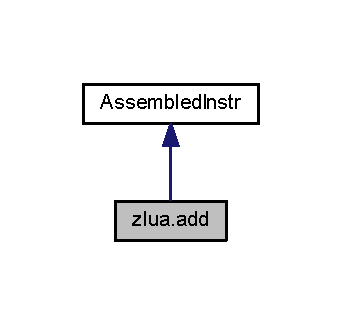
\includegraphics[width=164pt]{classzlua_1_1add__inherit__graph}
\end{center}
\end{figure}


Collaboration diagram for zlua.\+add\+:
\nopagebreak
\begin{figure}[H]
\begin{center}
\leavevmode
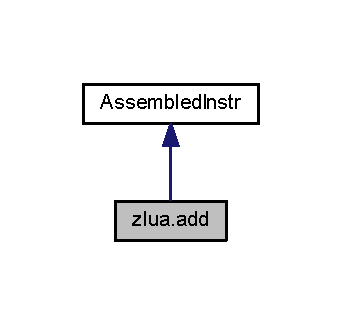
\includegraphics[width=164pt]{classzlua_1_1add__coll__graph}
\end{center}
\end{figure}
\subsection*{Public Member Functions}
\begin{DoxyCompactItemize}
\item 
override void \mbox{\hyperlink{classzlua_1_1add_a7a1a96e612bf700e73a640d4c4080179}{execute}} (\mbox{\hyperlink{classzlua_1_1lua___thread}{lua\+\_\+\+Thread}} thread)
\begin{DoxyCompactList}\small\item\em differ from py ver\+: C\# dont have meta programming, so must use polymorphic to implement visitor pattern and cause execution is in Instr env (I\+OC) \end{DoxyCompactList}\item 
\mbox{\Hypertarget{classzlua_1_1add_a85badfe9148e31edd2307a72be6d0757}\label{classzlua_1_1add_a85badfe9148e31edd2307a72be6d0757}} 
override string {\bfseries To\+String} ()
\end{DoxyCompactItemize}
\subsection*{Additional Inherited Members}


\subsection{Member Function Documentation}
\mbox{\Hypertarget{classzlua_1_1add_a7a1a96e612bf700e73a640d4c4080179}\label{classzlua_1_1add_a7a1a96e612bf700e73a640d4c4080179}} 
\index{zlua\+::add@{zlua\+::add}!execute@{execute}}
\index{execute@{execute}!zlua\+::add@{zlua\+::add}}
\subsubsection{\texorpdfstring{execute()}{execute()}}
{\footnotesize\ttfamily override void zlua.\+add.\+execute (\begin{DoxyParamCaption}\item[{\mbox{\hyperlink{classzlua_1_1lua___thread}{lua\+\_\+\+Thread}}}]{thread }\end{DoxyParamCaption})\hspace{0.3cm}{\ttfamily [virtual]}}



differ from py ver\+: C\# dont have meta programming, so must use polymorphic to implement visitor pattern and cause execution is in Instr env (I\+OC) 


\begin{DoxyParams}{Parameters}
{\em thread} & \\
\hline
\end{DoxyParams}


Implements \mbox{\hyperlink{classzlua_1_1_assembled_instr_a44e081c4565b90b75e4a67b8dd418feb}{zlua.\+Assembled\+Instr}}.



The documentation for this class was generated from the following file\+:\begin{DoxyCompactItemize}
\item 
zlua/I\+S\+A.\+cs\end{DoxyCompactItemize}

\hypertarget{classzlua_1_1and}{}\section{zlua.\+and Class Reference}
\label{classzlua_1_1and}\index{zlua.\+and@{zlua.\+and}}


Inheritance diagram for zlua.\+and\+:
\nopagebreak
\begin{figure}[H]
\begin{center}
\leavevmode
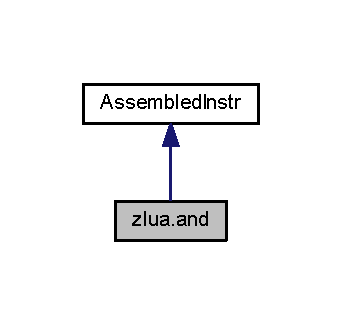
\includegraphics[width=164pt]{classzlua_1_1and__inherit__graph}
\end{center}
\end{figure}


Collaboration diagram for zlua.\+and\+:
\nopagebreak
\begin{figure}[H]
\begin{center}
\leavevmode
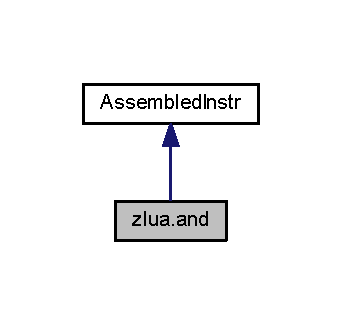
\includegraphics[width=164pt]{classzlua_1_1and__coll__graph}
\end{center}
\end{figure}
\subsection*{Public Member Functions}
\begin{DoxyCompactItemize}
\item 
override void \mbox{\hyperlink{classzlua_1_1and_ad1ef9d7bf03b778753264a15bbd6ac04}{execute}} (\mbox{\hyperlink{classzlua_1_1lua___thread}{lua\+\_\+\+Thread}} thread)
\begin{DoxyCompactList}\small\item\em differ from py ver\+: C\# dont have meta programming, so must use polymorphic to implement visitor pattern and cause execution is in Instr env (I\+OC) \end{DoxyCompactList}\item 
\mbox{\Hypertarget{classzlua_1_1and_aa49d463d28c5390025cfaf473c7cefd7}\label{classzlua_1_1and_aa49d463d28c5390025cfaf473c7cefd7}} 
override string {\bfseries To\+String} ()
\end{DoxyCompactItemize}
\subsection*{Additional Inherited Members}


\subsection{Member Function Documentation}
\mbox{\Hypertarget{classzlua_1_1and_ad1ef9d7bf03b778753264a15bbd6ac04}\label{classzlua_1_1and_ad1ef9d7bf03b778753264a15bbd6ac04}} 
\index{zlua\+::and@{zlua\+::and}!execute@{execute}}
\index{execute@{execute}!zlua\+::and@{zlua\+::and}}
\subsubsection{\texorpdfstring{execute()}{execute()}}
{\footnotesize\ttfamily override void zlua.\+and.\+execute (\begin{DoxyParamCaption}\item[{\mbox{\hyperlink{classzlua_1_1lua___thread}{lua\+\_\+\+Thread}}}]{thread }\end{DoxyParamCaption})\hspace{0.3cm}{\ttfamily [virtual]}}



differ from py ver\+: C\# dont have meta programming, so must use polymorphic to implement visitor pattern and cause execution is in Instr env (I\+OC) 


\begin{DoxyParams}{Parameters}
{\em thread} & \\
\hline
\end{DoxyParams}


Implements \mbox{\hyperlink{classzlua_1_1_assembled_instr_a44e081c4565b90b75e4a67b8dd418feb}{zlua.\+Assembled\+Instr}}.



The documentation for this class was generated from the following file\+:\begin{DoxyCompactItemize}
\item 
zlua/I\+S\+A.\+cs\end{DoxyCompactItemize}

\hypertarget{classzlua_1_1_assembled_instr}{}\section{zlua.\+Assembled\+Instr Class Reference}
\label{classzlua_1_1_assembled_instr}\index{zlua.\+Assembled\+Instr@{zlua.\+Assembled\+Instr}}


base class for all instructions  




Inheritance diagram for zlua.\+Assembled\+Instr\+:
\nopagebreak
\begin{figure}[H]
\begin{center}
\leavevmode
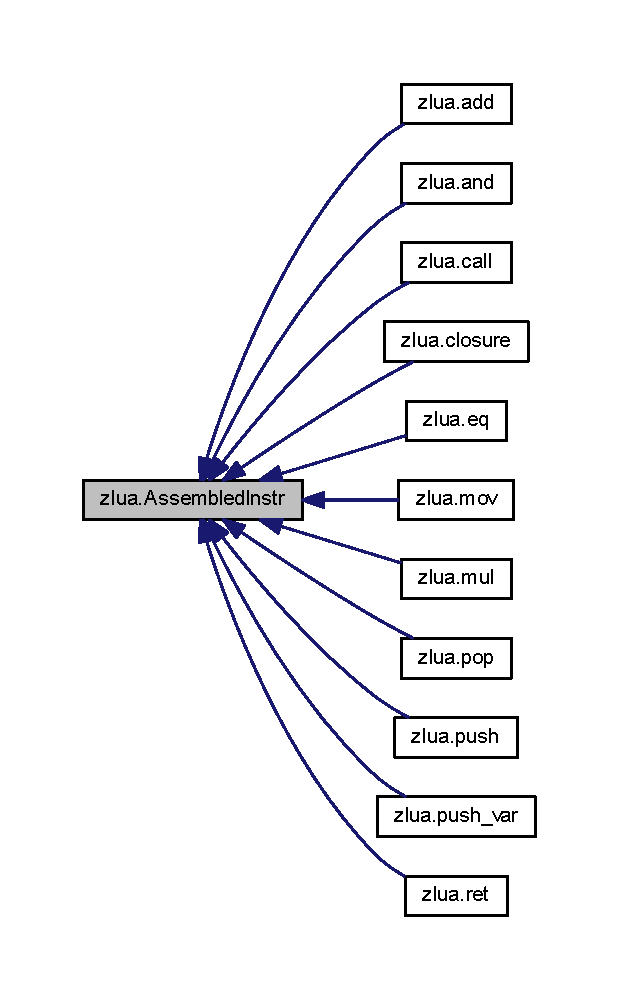
\includegraphics[width=297pt]{classzlua_1_1_assembled_instr__inherit__graph}
\end{center}
\end{figure}
\subsection*{Public Member Functions}
\begin{DoxyCompactItemize}
\item 
\mbox{\Hypertarget{classzlua_1_1_assembled_instr_a469a0a7a028bfa2bcc06920e1f6d45d6}\label{classzlua_1_1_assembled_instr_a469a0a7a028bfa2bcc06920e1f6d45d6}} 
abstract string {\bfseries To\+String} ()
\item 
abstract void \mbox{\hyperlink{classzlua_1_1_assembled_instr_a44e081c4565b90b75e4a67b8dd418feb}{execute}} (\mbox{\hyperlink{classzlua_1_1lua___thread}{lua\+\_\+\+Thread}} thread)
\begin{DoxyCompactList}\small\item\em differ from py ver\+: C\# dont have meta programming, so must use polymorphic to implement visitor pattern and cause execution is in Instr env (I\+OC) \end{DoxyCompactList}\end{DoxyCompactItemize}
\subsection*{Protected Attributes}
\begin{DoxyCompactItemize}
\item 
\mbox{\Hypertarget{classzlua_1_1_assembled_instr_a5adc24105bcb8588365861da83919070}\label{classzlua_1_1_assembled_instr_a5adc24105bcb8588365861da83919070}} 
List$<$ \mbox{\hyperlink{classzlua_1_1lua___t_value}{lua\+\_\+\+T\+Value}} $>$ {\bfseries operands} = new List$<$\mbox{\hyperlink{classzlua_1_1lua___t_value}{lua\+\_\+\+T\+Value}}$>$()
\end{DoxyCompactItemize}


\subsection{Detailed Description}
base class for all instructions 



\subsection{Member Function Documentation}
\mbox{\Hypertarget{classzlua_1_1_assembled_instr_a44e081c4565b90b75e4a67b8dd418feb}\label{classzlua_1_1_assembled_instr_a44e081c4565b90b75e4a67b8dd418feb}} 
\index{zlua\+::\+Assembled\+Instr@{zlua\+::\+Assembled\+Instr}!execute@{execute}}
\index{execute@{execute}!zlua\+::\+Assembled\+Instr@{zlua\+::\+Assembled\+Instr}}
\subsubsection{\texorpdfstring{execute()}{execute()}}
{\footnotesize\ttfamily abstract void zlua.\+Assembled\+Instr.\+execute (\begin{DoxyParamCaption}\item[{\mbox{\hyperlink{classzlua_1_1lua___thread}{lua\+\_\+\+Thread}}}]{thread }\end{DoxyParamCaption})\hspace{0.3cm}{\ttfamily [pure virtual]}}



differ from py ver\+: C\# dont have meta programming, so must use polymorphic to implement visitor pattern and cause execution is in Instr env (I\+OC) 


\begin{DoxyParams}{Parameters}
{\em thread} & \\
\hline
\end{DoxyParams}


Implemented in \mbox{\hyperlink{classzlua_1_1pop_a72cea959966aec69448d61be5bfc322c}{zlua.\+pop}}, \mbox{\hyperlink{classzlua_1_1push_ab3284599ae65d600d21622bd407405e8}{zlua.\+push}}, \mbox{\hyperlink{classzlua_1_1push__var_a854bc287123c636f0c3d86735938879f}{zlua.\+push\+\_\+var}}, \mbox{\hyperlink{classzlua_1_1and_ad1ef9d7bf03b778753264a15bbd6ac04}{zlua.\+and}}, \mbox{\hyperlink{classzlua_1_1eq_a802b2377436b97b137b50c36b2867d29}{zlua.\+eq}}, \mbox{\hyperlink{classzlua_1_1mul_a22002ab020aaabcf37eddae16b6ba10a}{zlua.\+mul}}, \mbox{\hyperlink{classzlua_1_1add_a7a1a96e612bf700e73a640d4c4080179}{zlua.\+add}}, \mbox{\hyperlink{classzlua_1_1ret_a0c334b18dbe8e21c26aa785269b29253}{zlua.\+ret}}, \mbox{\hyperlink{classzlua_1_1call_a152a4ccd3e77e5172f97283a50d6ba45}{zlua.\+call}}, \mbox{\hyperlink{classzlua_1_1closure_aa569159f1b1106362a86951524e96bce}{zlua.\+closure}}, and \mbox{\hyperlink{classzlua_1_1mov_a729d173bb798f765ed20aabcfaf2f63c}{zlua.\+mov}}.



The documentation for this class was generated from the following file\+:\begin{DoxyCompactItemize}
\item 
zlua/I\+S\+A.\+cs\end{DoxyCompactItemize}

\hypertarget{classzlua_1_1call}{}\section{zlua.\+call Class Reference}
\label{classzlua_1_1call}\index{zlua.\+call@{zlua.\+call}}


Inheritance diagram for zlua.\+call\+:
\nopagebreak
\begin{figure}[H]
\begin{center}
\leavevmode
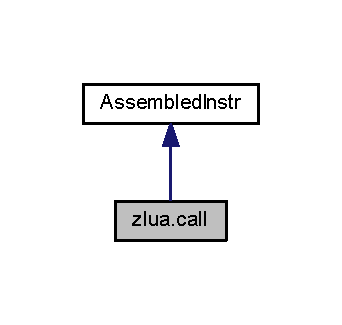
\includegraphics[width=164pt]{classzlua_1_1call__inherit__graph}
\end{center}
\end{figure}


Collaboration diagram for zlua.\+call\+:
\nopagebreak
\begin{figure}[H]
\begin{center}
\leavevmode
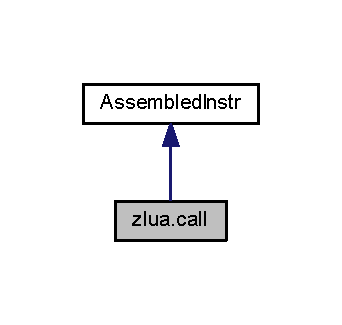
\includegraphics[width=164pt]{classzlua_1_1call__coll__graph}
\end{center}
\end{figure}
\subsection*{Public Member Functions}
\begin{DoxyCompactItemize}
\item 
\mbox{\Hypertarget{classzlua_1_1call_ac974a41a36538851e46c0dabe29e1769}\label{classzlua_1_1call_ac974a41a36538851e46c0dabe29e1769}} 
{\bfseries call} (string func\+\_\+name)
\item 
override void \mbox{\hyperlink{classzlua_1_1call_a152a4ccd3e77e5172f97283a50d6ba45}{execute}} (\mbox{\hyperlink{classzlua_1_1lua___thread}{lua\+\_\+\+Thread}} thread)
\begin{DoxyCompactList}\small\item\em differ from py ver\+: C\# dont have meta programming, so must use polymorphic to implement visitor pattern and cause execution is in Instr env (I\+OC) \end{DoxyCompactList}\item 
\mbox{\Hypertarget{classzlua_1_1call_a39377a59ffe57e46a5f7e930a50b4009}\label{classzlua_1_1call_a39377a59ffe57e46a5f7e930a50b4009}} 
override string {\bfseries To\+String} ()
\end{DoxyCompactItemize}
\subsection*{Additional Inherited Members}


\subsection{Member Function Documentation}
\mbox{\Hypertarget{classzlua_1_1call_a152a4ccd3e77e5172f97283a50d6ba45}\label{classzlua_1_1call_a152a4ccd3e77e5172f97283a50d6ba45}} 
\index{zlua\+::call@{zlua\+::call}!execute@{execute}}
\index{execute@{execute}!zlua\+::call@{zlua\+::call}}
\subsubsection{\texorpdfstring{execute()}{execute()}}
{\footnotesize\ttfamily override void zlua.\+call.\+execute (\begin{DoxyParamCaption}\item[{\mbox{\hyperlink{classzlua_1_1lua___thread}{lua\+\_\+\+Thread}}}]{thread }\end{DoxyParamCaption})\hspace{0.3cm}{\ttfamily [virtual]}}



differ from py ver\+: C\# dont have meta programming, so must use polymorphic to implement visitor pattern and cause execution is in Instr env (I\+OC) 


\begin{DoxyParams}{Parameters}
{\em thread} & \\
\hline
\end{DoxyParams}


Implements \mbox{\hyperlink{classzlua_1_1_assembled_instr_a44e081c4565b90b75e4a67b8dd418feb}{zlua.\+Assembled\+Instr}}.



The documentation for this class was generated from the following file\+:\begin{DoxyCompactItemize}
\item 
zlua/I\+S\+A.\+cs\end{DoxyCompactItemize}

\hypertarget{classzlua_1_1closure}{}\section{zlua.\+closure Class Reference}
\label{classzlua_1_1closure}\index{zlua.\+closure@{zlua.\+closure}}


Inheritance diagram for zlua.\+closure\+:
\nopagebreak
\begin{figure}[H]
\begin{center}
\leavevmode
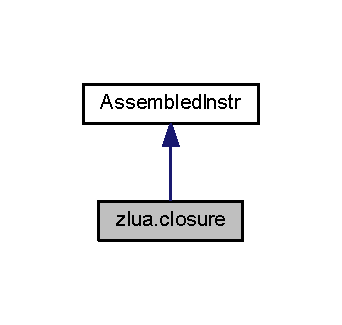
\includegraphics[width=164pt]{classzlua_1_1closure__inherit__graph}
\end{center}
\end{figure}


Collaboration diagram for zlua.\+closure\+:
\nopagebreak
\begin{figure}[H]
\begin{center}
\leavevmode
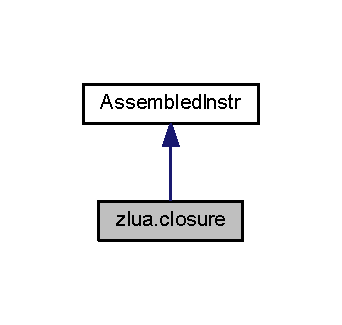
\includegraphics[width=164pt]{classzlua_1_1closure__coll__graph}
\end{center}
\end{figure}
\subsection*{Public Member Functions}
\begin{DoxyCompactItemize}
\item 
\mbox{\Hypertarget{classzlua_1_1closure_a42b516f075f4b4ce19e591d6102ca06c}\label{classzlua_1_1closure_a42b516f075f4b4ce19e591d6102ca06c}} 
{\bfseries closure} (int i)
\item 
override void \mbox{\hyperlink{classzlua_1_1closure_aa569159f1b1106362a86951524e96bce}{execute}} (\mbox{\hyperlink{classzlua_1_1lua___thread}{lua\+\_\+\+Thread}} thread)
\begin{DoxyCompactList}\small\item\em differ from py ver\+: C\# dont have meta programming, so must use polymorphic to implement visitor pattern and cause execution is in Instr env (I\+OC) \end{DoxyCompactList}\item 
\mbox{\Hypertarget{classzlua_1_1closure_a5ba32eccf1c70376f32ee6ca4bbe9424}\label{classzlua_1_1closure_a5ba32eccf1c70376f32ee6ca4bbe9424}} 
override string {\bfseries To\+String} ()
\end{DoxyCompactItemize}
\subsection*{Additional Inherited Members}


\subsection{Member Function Documentation}
\mbox{\Hypertarget{classzlua_1_1closure_aa569159f1b1106362a86951524e96bce}\label{classzlua_1_1closure_aa569159f1b1106362a86951524e96bce}} 
\index{zlua\+::closure@{zlua\+::closure}!execute@{execute}}
\index{execute@{execute}!zlua\+::closure@{zlua\+::closure}}
\subsubsection{\texorpdfstring{execute()}{execute()}}
{\footnotesize\ttfamily override void zlua.\+closure.\+execute (\begin{DoxyParamCaption}\item[{\mbox{\hyperlink{classzlua_1_1lua___thread}{lua\+\_\+\+Thread}}}]{thread }\end{DoxyParamCaption})\hspace{0.3cm}{\ttfamily [virtual]}}



differ from py ver\+: C\# dont have meta programming, so must use polymorphic to implement visitor pattern and cause execution is in Instr env (I\+OC) 


\begin{DoxyParams}{Parameters}
{\em thread} & \\
\hline
\end{DoxyParams}


Implements \mbox{\hyperlink{classzlua_1_1_assembled_instr_a44e081c4565b90b75e4a67b8dd418feb}{zlua.\+Assembled\+Instr}}.



The documentation for this class was generated from the following file\+:\begin{DoxyCompactItemize}
\item 
zlua/I\+S\+A.\+cs\end{DoxyCompactItemize}

\hypertarget{classzlua_1_1_compiled_function}{}\section{zlua.\+Compiled\+Function Class Reference}
\label{classzlua_1_1_compiled_function}\index{zlua.\+Compiled\+Function@{zlua.\+Compiled\+Function}}


\char`\"{}\+Proto in lua.\+c\char`\"{} proto is gcobject, but is not a primitive type  




Inheritance diagram for zlua.\+Compiled\+Function\+:
\nopagebreak
\begin{figure}[H]
\begin{center}
\leavevmode
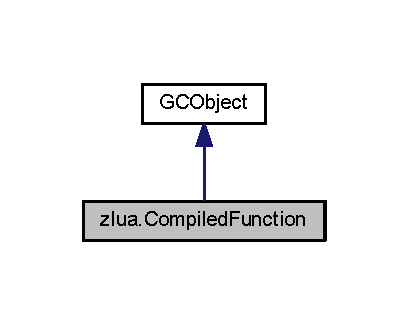
\includegraphics[width=196pt]{classzlua_1_1_compiled_function__inherit__graph}
\end{center}
\end{figure}


Collaboration diagram for zlua.\+Compiled\+Function\+:
\nopagebreak
\begin{figure}[H]
\begin{center}
\leavevmode
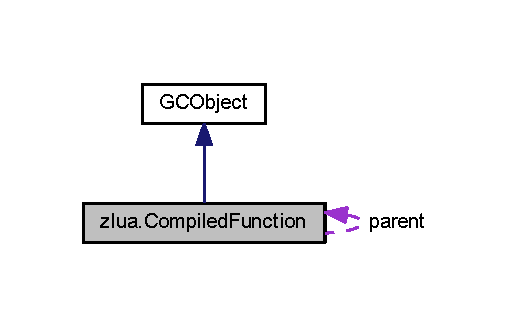
\includegraphics[width=245pt]{classzlua_1_1_compiled_function__coll__graph}
\end{center}
\end{figure}
\subsection*{Public Member Functions}
\begin{DoxyCompactItemize}
\item 
\mbox{\Hypertarget{classzlua_1_1_compiled_function_ab75dd80d0ff208969ee9cd9dd56cd2d6}\label{classzlua_1_1_compiled_function_ab75dd80d0ff208969ee9cd9dd56cd2d6}} 
{\bfseries Compiled\+Function} (\mbox{\hyperlink{classzlua_1_1_compiled_function}{Compiled\+Function}} parent, List$<$ string $>$ param\+\_\+names)
\end{DoxyCompactItemize}
\subsection*{Public Attributes}
\begin{DoxyCompactItemize}
\item 
\mbox{\Hypertarget{classzlua_1_1_compiled_function_a1f6f1c48793a163d632ea42d5a5693b4}\label{classzlua_1_1_compiled_function_a1f6f1c48793a163d632ea42d5a5693b4}} 
List$<$ string $>$ {\bfseries param\+\_\+names}
\item 
\mbox{\Hypertarget{classzlua_1_1_compiled_function_a503d3c1785d7bfa6c9397db569c6e09e}\label{classzlua_1_1_compiled_function_a503d3c1785d7bfa6c9397db569c6e09e}} 
\mbox{\hyperlink{classzlua_1_1_compiled_function}{Compiled\+Function}} {\bfseries parent}
\item 
\mbox{\Hypertarget{classzlua_1_1_compiled_function_a30fd2db9dbd3e461f92f86928130d514}\label{classzlua_1_1_compiled_function_a30fd2db9dbd3e461f92f86928130d514}} 
List$<$ \mbox{\hyperlink{classzlua_1_1_assembled_instr}{Assembled\+Instr}} $>$ {\bfseries instrs} = new List$<$\mbox{\hyperlink{classzlua_1_1_assembled_instr}{Assembled\+Instr}}$>$()
\item 
\mbox{\Hypertarget{classzlua_1_1_compiled_function_aa4fd3601855cf91d034a2d4ff43b7a75}\label{classzlua_1_1_compiled_function_aa4fd3601855cf91d034a2d4ff43b7a75}} 
List$<$ \mbox{\hyperlink{classzlua_1_1_compiled_function}{Compiled\+Function}} $>$ {\bfseries inner\+\_\+funcs} = new List$<$\mbox{\hyperlink{classzlua_1_1_compiled_function}{Compiled\+Function}}$>$()
\item 
\mbox{\Hypertarget{classzlua_1_1_compiled_function_ab4bc14259fb6e1e10152f6a0d766f143}\label{classzlua_1_1_compiled_function_ab4bc14259fb6e1e10152f6a0d766f143}} 
Dictionary$<$ string, int $>$ {\bfseries label2pc} = new Dictionary$<$string, int$>$()
\end{DoxyCompactItemize}
\subsection*{Additional Inherited Members}


\subsection{Detailed Description}
\char`\"{}\+Proto in lua.\+c\char`\"{} proto is gcobject, but is not a primitive type 



The documentation for this class was generated from the following file\+:\begin{DoxyCompactItemize}
\item 
zlua/lobject.\+cs\end{DoxyCompactItemize}

\hypertarget{classzlua_1_1eq}{}\section{zlua.\+eq Class Reference}
\label{classzlua_1_1eq}\index{zlua.\+eq@{zlua.\+eq}}


Inheritance diagram for zlua.\+eq\+:
\nopagebreak
\begin{figure}[H]
\begin{center}
\leavevmode
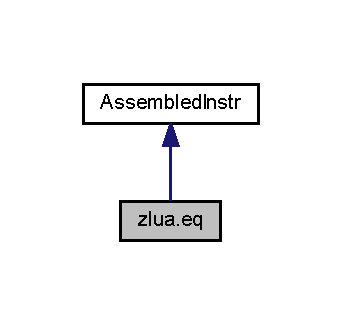
\includegraphics[width=164pt]{classzlua_1_1eq__inherit__graph}
\end{center}
\end{figure}


Collaboration diagram for zlua.\+eq\+:
\nopagebreak
\begin{figure}[H]
\begin{center}
\leavevmode
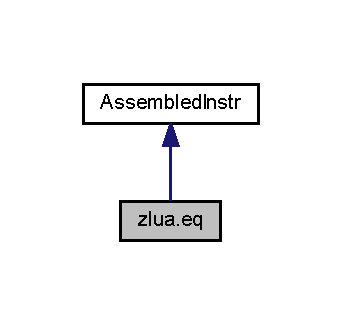
\includegraphics[width=164pt]{classzlua_1_1eq__coll__graph}
\end{center}
\end{figure}
\subsection*{Public Member Functions}
\begin{DoxyCompactItemize}
\item 
override void \mbox{\hyperlink{classzlua_1_1eq_a802b2377436b97b137b50c36b2867d29}{execute}} (\mbox{\hyperlink{classzlua_1_1lua___thread}{lua\+\_\+\+Thread}} thread)
\begin{DoxyCompactList}\small\item\em differ from py ver\+: C\# dont have meta programming, so must use polymorphic to implement visitor pattern and cause execution is in Instr env (I\+OC) \end{DoxyCompactList}\item 
\mbox{\Hypertarget{classzlua_1_1eq_a556330ea93d3dc16291681a1ece7d3a7}\label{classzlua_1_1eq_a556330ea93d3dc16291681a1ece7d3a7}} 
override string {\bfseries To\+String} ()
\end{DoxyCompactItemize}
\subsection*{Additional Inherited Members}


\subsection{Member Function Documentation}
\mbox{\Hypertarget{classzlua_1_1eq_a802b2377436b97b137b50c36b2867d29}\label{classzlua_1_1eq_a802b2377436b97b137b50c36b2867d29}} 
\index{zlua\+::eq@{zlua\+::eq}!execute@{execute}}
\index{execute@{execute}!zlua\+::eq@{zlua\+::eq}}
\subsubsection{\texorpdfstring{execute()}{execute()}}
{\footnotesize\ttfamily override void zlua.\+eq.\+execute (\begin{DoxyParamCaption}\item[{\mbox{\hyperlink{classzlua_1_1lua___thread}{lua\+\_\+\+Thread}}}]{thread }\end{DoxyParamCaption})\hspace{0.3cm}{\ttfamily [virtual]}}



differ from py ver\+: C\# dont have meta programming, so must use polymorphic to implement visitor pattern and cause execution is in Instr env (I\+OC) 


\begin{DoxyParams}{Parameters}
{\em thread} & \\
\hline
\end{DoxyParams}


Implements \mbox{\hyperlink{classzlua_1_1_assembled_instr_a44e081c4565b90b75e4a67b8dd418feb}{zlua.\+Assembled\+Instr}}.



The documentation for this class was generated from the following file\+:\begin{DoxyCompactItemize}
\item 
zlua/I\+S\+A.\+cs\end{DoxyCompactItemize}

\hypertarget{classzlua_1_1_g_c_object}{}\section{zlua.\+G\+C\+Object Class Reference}
\label{classzlua_1_1_g_c_object}\index{zlua.\+G\+C\+Object@{zlua.\+G\+C\+Object}}


(C\# simulated) union of GC objects how it simulates union\+: polymorphic  




Inheritance diagram for zlua.\+G\+C\+Object\+:
\nopagebreak
\begin{figure}[H]
\begin{center}
\leavevmode
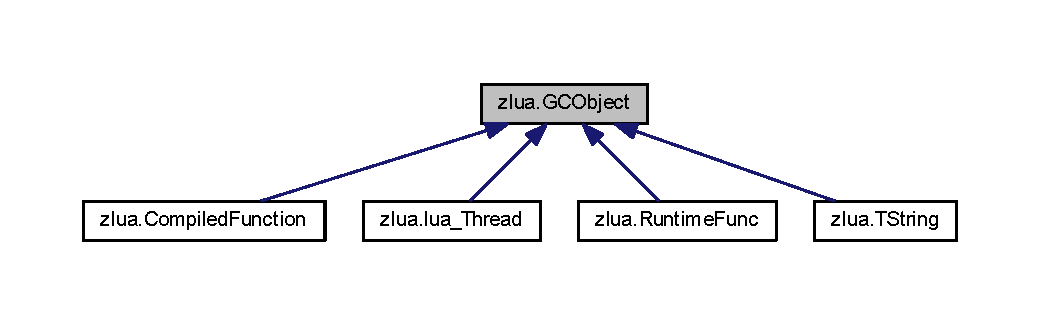
\includegraphics[width=350pt]{classzlua_1_1_g_c_object__inherit__graph}
\end{center}
\end{figure}
\subsection*{Properties}
\begin{DoxyCompactItemize}
\item 
\mbox{\hyperlink{classzlua_1_1_t_string}{T\+String}} \mbox{\hyperlink{classzlua_1_1_g_c_object_adcdbddfaf950e2317f916f184d5b9cfb}{tstring}}\hspace{0.3cm}{\ttfamily  \mbox{[}get\mbox{]}}
\begin{DoxyCompactList}\small\item\em for convenience (eg. \mbox{\hyperlink{classzlua_1_1_t_string}{T\+String}} is subclass of G\+C\+Object) \end{DoxyCompactList}\item 
\mbox{\Hypertarget{classzlua_1_1_g_c_object_a7146f38e63ed0b5ce02b3df6018593cd}\label{classzlua_1_1_g_c_object_a7146f38e63ed0b5ce02b3df6018593cd}} 
\mbox{\hyperlink{classzlua_1_1lua___thread}{lua\+\_\+\+Thread}} {\bfseries thread}\hspace{0.3cm}{\ttfamily  \mbox{[}get\mbox{]}}
\item 
\mbox{\Hypertarget{classzlua_1_1_g_c_object_a0310e8bc45b59801052df6a32dcaa123}\label{classzlua_1_1_g_c_object_a0310e8bc45b59801052df6a32dcaa123}} 
\mbox{\hyperlink{classzlua_1_1_compiled_function}{Compiled\+Function}} {\bfseries compiled\+\_\+func}\hspace{0.3cm}{\ttfamily  \mbox{[}get\mbox{]}}
\item 
\mbox{\Hypertarget{classzlua_1_1_g_c_object_aaff4acdded9ec0227d9837632498d32c}\label{classzlua_1_1_g_c_object_aaff4acdded9ec0227d9837632498d32c}} 
\mbox{\hyperlink{classzlua_1_1_runtime_func}{Runtime\+Func}} {\bfseries runtime\+\_\+func}\hspace{0.3cm}{\ttfamily  \mbox{[}get\mbox{]}}
\end{DoxyCompactItemize}


\subsection{Detailed Description}
(C\# simulated) union of GC objects how it simulates union\+: polymorphic 


\begin{DoxyEnumerate}
\item inheritance graph\+: G\+Cheader $>$ \mbox{\hyperlink{classzlua_1_1_g_c_object}{G\+C\+Object}} $>$ \mbox{\hyperlink{classzlua_1_1_t_string}{T\+String}}, Udata ... (all GC types of lua)
\item \mbox{\hyperlink{classzlua_1_1_g_c_object}{G\+C\+Object}} use property to return specific type of value with polymorphic 
\end{DoxyEnumerate}

\subsection{Property Documentation}
\mbox{\Hypertarget{classzlua_1_1_g_c_object_adcdbddfaf950e2317f916f184d5b9cfb}\label{classzlua_1_1_g_c_object_adcdbddfaf950e2317f916f184d5b9cfb}} 
\index{zlua\+::\+G\+C\+Object@{zlua\+::\+G\+C\+Object}!tstring@{tstring}}
\index{tstring@{tstring}!zlua\+::\+G\+C\+Object@{zlua\+::\+G\+C\+Object}}
\subsubsection{\texorpdfstring{tstring}{tstring}}
{\footnotesize\ttfamily \mbox{\hyperlink{classzlua_1_1_t_string}{T\+String}} zlua.\+G\+C\+Object.\+tstring\hspace{0.3cm}{\ttfamily [get]}}



for convenience (eg. \mbox{\hyperlink{classzlua_1_1_t_string}{T\+String}} is subclass of G\+C\+Object) 



The documentation for this class was generated from the following file\+:\begin{DoxyCompactItemize}
\item 
zlua/lobject.\+cs\end{DoxyCompactItemize}

\hypertarget{classzlua_1_1_lua}{}\section{zlua.\+Lua Class Reference}
\label{classzlua_1_1_lua}\index{zlua.\+Lua@{zlua.\+Lua}}


some generic functions over lua objects (lobject.\+c)  


\subsection*{Classes}
\begin{DoxyCompactItemize}
\item 
class \mbox{\hyperlink{classzlua_1_1_lua_1_1_assembled_instr}{Assembled\+Instr}}
\item 
class \mbox{\hyperlink{classzlua_1_1_lua_1_1_compiled_function}{Compiled\+Function}}
\begin{DoxyCompactList}\small\item\em \char`\"{}\+Proto in lua.\+c\char`\"{} proto is gcobject, but is not a primitive type \end{DoxyCompactList}\item 
class \mbox{\hyperlink{classzlua_1_1_lua_1_1_g_c_object}{G\+C\+Object}}
\begin{DoxyCompactList}\small\item\em (C\# simulated) union of GC objects how it simulates union\+: polymorphic \end{DoxyCompactList}\item 
class \mbox{\hyperlink{classzlua_1_1_lua_1_1lua___t_value}{lua\+\_\+\+T\+Value}}
\begin{DoxyCompactList}\small\item\em the general type of lua. T means \char`\"{}tagged\char`\"{} \end{DoxyCompactList}\item 
class \mbox{\hyperlink{classzlua_1_1_lua_1_1_runtime_func}{Runtime\+Func}}
\begin{DoxyCompactList}\small\item\em \char`\"{}\+Clousure\char`\"{} in lua.\+c \end{DoxyCompactList}\item 
class \mbox{\hyperlink{classzlua_1_1_lua_1_1_t_string}{T\+String}}
\begin{DoxyCompactList}\small\item\em the string type of lua, just warpper of C\# string \end{DoxyCompactList}\item 
class \mbox{\hyperlink{classzlua_1_1_lua_1_1_value}{Value}}
\begin{DoxyCompactList}\small\item\em (C\# simulated) union of all lua values how it simulate union?\+: use extra fields size\+: 8+8+4=20B differ from clua\+: light userdata is removed because C\# use GC T\+O\+D\+O如何访问修饰符不被外卖呢看到 \end{DoxyCompactList}\end{DoxyCompactItemize}
\subsection*{Public Types}
\begin{DoxyCompactItemize}
\item 
enum \mbox{\hyperlink{classzlua_1_1_lua_a3bea46ecc2aabf23ac160bd7e7172e70}{Lua\+Type}} \{ \newline
{\bfseries N\+O\+NE} = -\/1, 
{\bfseries N\+IL} = 0, 
{\bfseries B\+O\+O\+L\+E\+AN} = 1, 
{\bfseries L\+I\+G\+H\+T\+U\+S\+E\+R\+D\+A\+TA} = 2, 
\newline
{\bfseries N\+U\+M\+B\+ER} = 3, 
{\bfseries S\+T\+R\+I\+NG} = 4, 
{\bfseries T\+A\+B\+LE} = 5, 
{\bfseries F\+U\+N\+C\+T\+I\+ON} = 6, 
\newline
{\bfseries U\+S\+E\+R\+D\+A\+TA} = 7, 
{\bfseries T\+H\+R\+E\+AD} = 8
 \}
\begin{DoxyCompactList}\small\item\em differ from clua\+: const int... =$>$ enum \end{DoxyCompactList}\end{DoxyCompactItemize}
\subsection*{Public Member Functions}
\begin{DoxyCompactItemize}
\item 
\mbox{\Hypertarget{classzlua_1_1_lua_a8d69f72236b14935e2f4da7360dfc00f}\label{classzlua_1_1_lua_a8d69f72236b14935e2f4da7360dfc00f}} 
void {\bfseries dofile} (string path)
\end{DoxyCompactItemize}


\subsection{Detailed Description}
some generic functions over lua objects (lobject.\+c) 

vm 

lua对外接口,类型和dofile等等(lua.\+c in lua src) 


\begin{DoxyEnumerate}
\item interface\mbox{]} T\+Value, and other 9 specific types ~\newline
2. G\+C不实现,使用C\# GC 
\end{DoxyEnumerate}

\subsection{Member Enumeration Documentation}
\mbox{\Hypertarget{classzlua_1_1_lua_a3bea46ecc2aabf23ac160bd7e7172e70}\label{classzlua_1_1_lua_a3bea46ecc2aabf23ac160bd7e7172e70}} 
\index{zlua\+::\+Lua@{zlua\+::\+Lua}!Lua\+Type@{Lua\+Type}}
\index{Lua\+Type@{Lua\+Type}!zlua\+::\+Lua@{zlua\+::\+Lua}}
\subsubsection{\texorpdfstring{Lua\+Type}{LuaType}}
{\footnotesize\ttfamily enum \mbox{\hyperlink{classzlua_1_1_lua_a3bea46ecc2aabf23ac160bd7e7172e70}{zlua.\+Lua.\+Lua\+Type}}\hspace{0.3cm}{\ttfamily [strong]}}



differ from clua\+: const int... =$>$ enum 



The documentation for this class was generated from the following files\+:\begin{DoxyCompactItemize}
\item 
zlua/lobject.\+cs\item 
zlua/lua.\+cs\end{DoxyCompactItemize}

\hypertarget{classzlua_1_1lua___thread}{}\section{zlua.\+lua\+\_\+\+Thread Class Reference}
\label{classzlua_1_1lua___thread}\index{zlua.\+lua\+\_\+\+Thread@{zlua.\+lua\+\_\+\+Thread}}


Inheritance diagram for zlua.\+lua\+\_\+\+Thread\+:
\nopagebreak
\begin{figure}[H]
\begin{center}
\leavevmode
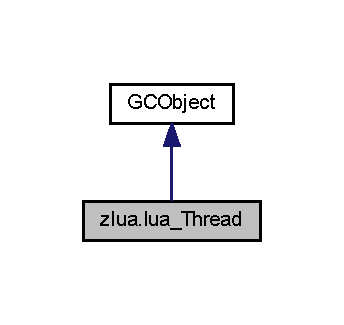
\includegraphics[width=165pt]{classzlua_1_1lua___thread__inherit__graph}
\end{center}
\end{figure}


Collaboration diagram for zlua.\+lua\+\_\+\+Thread\+:
\nopagebreak
\begin{figure}[H]
\begin{center}
\leavevmode
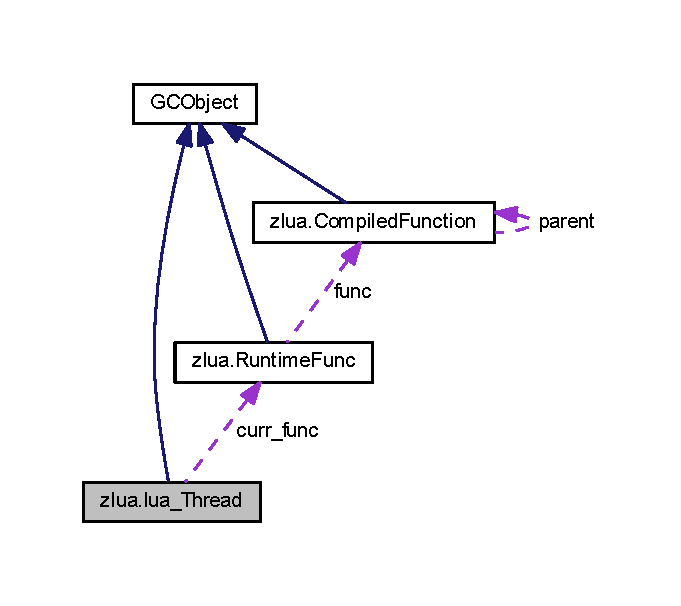
\includegraphics[width=327pt]{classzlua_1_1lua___thread__coll__graph}
\end{center}
\end{figure}
\subsection*{Public Member Functions}
\begin{DoxyCompactItemize}
\item 
\mbox{\Hypertarget{classzlua_1_1lua___thread_a636e6a5c2880d7d5c5b82284122dd46c}\label{classzlua_1_1lua___thread_a636e6a5c2880d7d5c5b82284122dd46c}} 
{\bfseries lua\+\_\+\+Thread} (\mbox{\hyperlink{classzlua_1_1_compiled_function}{Compiled\+Function}} main\+\_\+func)
\item 
\mbox{\Hypertarget{classzlua_1_1lua___thread_a97db462cd29e287ac92aaa4e4e189cf9}\label{classzlua_1_1lua___thread_a97db462cd29e287ac92aaa4e4e189cf9}} 
void {\bfseries run} ()
\item 
\mbox{\Hypertarget{classzlua_1_1lua___thread_aef81d9d2f99814679589de928a169dc1}\label{classzlua_1_1lua___thread_aef81d9d2f99814679589de928a169dc1}} 
void {\bfseries push} (\mbox{\hyperlink{classzlua_1_1lua___t_value}{lua\+\_\+\+T\+Value}} item)
\item 
\mbox{\Hypertarget{classzlua_1_1lua___thread_a6bea0e6f7b063a4c2c7b66e3ea152d31}\label{classzlua_1_1lua___thread_a6bea0e6f7b063a4c2c7b66e3ea152d31}} 
\mbox{\hyperlink{classzlua_1_1lua___t_value}{lua\+\_\+\+T\+Value}} {\bfseries pop} ()
\end{DoxyCompactItemize}
\subsection*{Public Attributes}
\begin{DoxyCompactItemize}
\item 
\mbox{\Hypertarget{classzlua_1_1lua___thread_ac75eedf89c86746fddf420372c1ba7b8}\label{classzlua_1_1lua___thread_ac75eedf89c86746fddf420372c1ba7b8}} 
Stack$<$ \mbox{\hyperlink{classzlua_1_1_runtime_func}{Runtime\+Func}} $>$ {\bfseries stack} = new Stack$<$\mbox{\hyperlink{classzlua_1_1_runtime_func}{Runtime\+Func}}$>$()
\item 
\mbox{\Hypertarget{classzlua_1_1lua___thread_a6dbf42b795dc65215c8f04958901bbee}\label{classzlua_1_1lua___thread_a6dbf42b795dc65215c8f04958901bbee}} 
Dictionary$<$ string, \mbox{\hyperlink{classzlua_1_1lua___t_value}{lua\+\_\+\+T\+Value}} $>$ {\bfseries global\+\_\+data}
\item 
\mbox{\Hypertarget{classzlua_1_1lua___thread_ab35e12bb7ab159fdef6ea7cb8548875d}\label{classzlua_1_1lua___thread_ab35e12bb7ab159fdef6ea7cb8548875d}} 
int {\bfseries pc} = 0
\item 
\mbox{\Hypertarget{classzlua_1_1lua___thread_a826cce1f5eb8ad00973c8d4c4cda6754}\label{classzlua_1_1lua___thread_a826cce1f5eb8ad00973c8d4c4cda6754}} 
\mbox{\hyperlink{classzlua_1_1_runtime_func}{Runtime\+Func}} {\bfseries curr\+\_\+func} =$>$ stack.\+Peek()
\end{DoxyCompactItemize}
\subsection*{Additional Inherited Members}


The documentation for this class was generated from the following file\+:\begin{DoxyCompactItemize}
\item 
zlua/lvm.\+cs\end{DoxyCompactItemize}

\hypertarget{classzlua_1_1lua___t_value}{}\section{zlua.\+lua\+\_\+\+T\+Value Class Reference}
\label{classzlua_1_1lua___t_value}\index{zlua.\+lua\+\_\+\+T\+Value@{zlua.\+lua\+\_\+\+T\+Value}}


the general type of lua. T means \char`\"{}tagged\char`\"{} methods brief\+:  


\subsection*{Public Member Functions}
\begin{DoxyCompactItemize}
\item 
\mbox{\Hypertarget{classzlua_1_1lua___t_value_a20dbc4df0c9bccde32812725fab7a2b3}\label{classzlua_1_1lua___t_value_a20dbc4df0c9bccde32812725fab7a2b3}} 
override string {\bfseries To\+String} ()
\item 
\mbox{\Hypertarget{classzlua_1_1lua___t_value_a0405a3303a63c8dc69fd27fc7739b23f}\label{classzlua_1_1lua___t_value_a0405a3303a63c8dc69fd27fc7739b23f}} 
bool {\bfseries is\+\_\+tstring} ()
\end{DoxyCompactItemize}
\subsection*{Static Public Member Functions}
\begin{DoxyCompactItemize}
\item 
\mbox{\Hypertarget{classzlua_1_1lua___t_value_a9b0783880dcd50991ac1f6abb71f5c25}\label{classzlua_1_1lua___t_value_a9b0783880dcd50991ac1f6abb71f5c25}} 
static \mbox{\hyperlink{classzlua_1_1lua___t_value}{lua\+\_\+\+T\+Value}} {\bfseries nil\+\_\+factory} ()
\item 
\mbox{\Hypertarget{classzlua_1_1lua___t_value_a8bd4399873075abd5d6610da5966a171}\label{classzlua_1_1lua___t_value_a8bd4399873075abd5d6610da5966a171}} 
static \mbox{\hyperlink{classzlua_1_1lua___t_value}{lua\+\_\+\+T\+Value}} {\bfseries tstring\+\_\+factory} (string s)
\item 
\mbox{\Hypertarget{classzlua_1_1lua___t_value_a8a92c76819e7f16495848cbc6daf6c25}\label{classzlua_1_1lua___t_value_a8a92c76819e7f16495848cbc6daf6c25}} 
static \mbox{\hyperlink{classzlua_1_1lua___t_value}{lua\+\_\+\+T\+Value}} {\bfseries runtime\+\_\+func\+\_\+factory} (\mbox{\hyperlink{classzlua_1_1_compiled_function}{Compiled\+Function}} func)
\item 
\mbox{\Hypertarget{classzlua_1_1lua___t_value_a21f1aa815c2d630491ea1972eb89b789}\label{classzlua_1_1lua___t_value_a21f1aa815c2d630491ea1972eb89b789}} 
static \mbox{\hyperlink{classzlua_1_1lua___t_value}{lua\+\_\+\+T\+Value}} {\bfseries bool\+\_\+factory} (bool b)
\item 
\mbox{\Hypertarget{classzlua_1_1lua___t_value_a8027e82c713365a731fc06433a326b95}\label{classzlua_1_1lua___t_value_a8027e82c713365a731fc06433a326b95}} 
static \mbox{\hyperlink{classzlua_1_1lua___t_value}{lua\+\_\+\+T\+Value}} {\bfseries compiled\+\_\+func\+\_\+factory} (\mbox{\hyperlink{classzlua_1_1_compiled_function}{Compiled\+Function}} compiled\+Function)
\item 
\mbox{\Hypertarget{classzlua_1_1lua___t_value_afc07e7986c5c9b9b39994222f19e8be6}\label{classzlua_1_1lua___t_value_afc07e7986c5c9b9b39994222f19e8be6}} 
static \mbox{\hyperlink{classzlua_1_1lua___t_value}{lua\+\_\+\+T\+Value}} {\bfseries i\+\_\+factory} (int i)
\item 
\mbox{\Hypertarget{classzlua_1_1lua___t_value_ac953d7451177d288a1d82026049bc2ae}\label{classzlua_1_1lua___t_value_ac953d7451177d288a1d82026049bc2ae}} 
static \mbox{\hyperlink{classzlua_1_1lua___t_value}{lua\+\_\+\+T\+Value}} {\bfseries operator+} (\mbox{\hyperlink{classzlua_1_1lua___t_value}{lua\+\_\+\+T\+Value}} lhs, \mbox{\hyperlink{classzlua_1_1lua___t_value}{lua\+\_\+\+T\+Value}} rhs)
\item 
\mbox{\Hypertarget{classzlua_1_1lua___t_value_a3b8dee11d04c27073957a77f875565c9}\label{classzlua_1_1lua___t_value_a3b8dee11d04c27073957a77f875565c9}} 
static \mbox{\hyperlink{classzlua_1_1lua___t_value}{lua\+\_\+\+T\+Value}} {\bfseries n\+\_\+factory} (lua\+\_\+\+Number n)
\item 
\mbox{\Hypertarget{classzlua_1_1lua___t_value_a9552f9ca3c36ef70355b610e0956fdca}\label{classzlua_1_1lua___t_value_a9552f9ca3c36ef70355b610e0956fdca}} 
static \mbox{\hyperlink{classzlua_1_1lua___t_value}{lua\+\_\+\+T\+Value}} {\bfseries operator$\ast$} (\mbox{\hyperlink{classzlua_1_1lua___t_value}{lua\+\_\+\+T\+Value}} lhs, \mbox{\hyperlink{classzlua_1_1lua___t_value}{lua\+\_\+\+T\+Value}} rhs)
\item 
\mbox{\Hypertarget{classzlua_1_1lua___t_value_a8a92d8894ed23f4b1ca41320ce32afeb}\label{classzlua_1_1lua___t_value_a8a92d8894ed23f4b1ca41320ce32afeb}} 
static \mbox{\hyperlink{classzlua_1_1lua___t_value}{lua\+\_\+\+T\+Value}} {\bfseries and} (\mbox{\hyperlink{classzlua_1_1lua___t_value}{lua\+\_\+\+T\+Value}} lhs, \mbox{\hyperlink{classzlua_1_1lua___t_value}{lua\+\_\+\+T\+Value}} rhs)
\item 
\mbox{\Hypertarget{classzlua_1_1lua___t_value_a2e76bff40e560afe1237dd5d27956f7d}\label{classzlua_1_1lua___t_value_a2e76bff40e560afe1237dd5d27956f7d}} 
static \mbox{\hyperlink{classzlua_1_1lua___t_value}{lua\+\_\+\+T\+Value}} {\bfseries eq} (\mbox{\hyperlink{classzlua_1_1lua___t_value}{lua\+\_\+\+T\+Value}} lhs, \mbox{\hyperlink{classzlua_1_1lua___t_value}{lua\+\_\+\+T\+Value}} rhs)
\item 
\mbox{\Hypertarget{classzlua_1_1lua___t_value_ab201201cd8bc483fa6e6fa04156e5fe2}\label{classzlua_1_1lua___t_value_ab201201cd8bc483fa6e6fa04156e5fe2}} 
static \mbox{\hyperlink{classzlua_1_1lua___t_value}{lua\+\_\+\+T\+Value}} {\bfseries b\+\_\+factory} (bool b)
\end{DoxyCompactItemize}
\subsection*{Properties}
\begin{DoxyCompactItemize}
\item 
\mbox{\Hypertarget{classzlua_1_1lua___t_value_a1b3b6cb5930ef892d5ec7fa8d3421b30}\label{classzlua_1_1lua___t_value_a1b3b6cb5930ef892d5ec7fa8d3421b30}} 
string {\bfseries str}\hspace{0.3cm}{\ttfamily  \mbox{[}get\mbox{]}}
\item 
\mbox{\Hypertarget{classzlua_1_1lua___t_value_af86fc5ea154a68a65fef269dc28a5799}\label{classzlua_1_1lua___t_value_af86fc5ea154a68a65fef269dc28a5799}} 
\mbox{\hyperlink{classzlua_1_1_compiled_function}{Compiled\+Function}} {\bfseries compiled\+\_\+func}\hspace{0.3cm}{\ttfamily  \mbox{[}get\mbox{]}}
\item 
\mbox{\Hypertarget{classzlua_1_1lua___t_value_afaa893cd000573cc850bea3fbc51825a}\label{classzlua_1_1lua___t_value_afaa893cd000573cc850bea3fbc51825a}} 
int {\bfseries i}\hspace{0.3cm}{\ttfamily  \mbox{[}get\mbox{]}}
\item 
\mbox{\Hypertarget{classzlua_1_1lua___t_value_aac7abef92780df48bf961a2ea54440d3}\label{classzlua_1_1lua___t_value_aac7abef92780df48bf961a2ea54440d3}} 
lua\+\_\+\+Number {\bfseries n}\hspace{0.3cm}{\ttfamily  \mbox{[}get\mbox{]}}
\item 
\mbox{\Hypertarget{classzlua_1_1lua___t_value_a76fd6fe1760b731a9e9e0662384b2a0e}\label{classzlua_1_1lua___t_value_a76fd6fe1760b731a9e9e0662384b2a0e}} 
bool {\bfseries b}\hspace{0.3cm}{\ttfamily  \mbox{[}get\mbox{]}}
\end{DoxyCompactItemize}


\subsection{Detailed Description}
the general type of lua. T means \char`\"{}tagged\char`\"{} methods brief\+: 


\begin{DoxyEnumerate}
\item factory\+: return a new specified lua type value; cast C\# type to lua type (eg. string =$>$ tstring)
\item property\+: get, set a specified lua type value
\item cast among lua types is not needed 
\end{DoxyEnumerate}

The documentation for this class was generated from the following file\+:\begin{DoxyCompactItemize}
\item 
zlua/lobject.\+cs\end{DoxyCompactItemize}

\hypertarget{classzlua_1_1mov}{}\section{zlua.\+mov Class Reference}
\label{classzlua_1_1mov}\index{zlua.\+mov@{zlua.\+mov}}


Inheritance diagram for zlua.\+mov\+:
\nopagebreak
\begin{figure}[H]
\begin{center}
\leavevmode
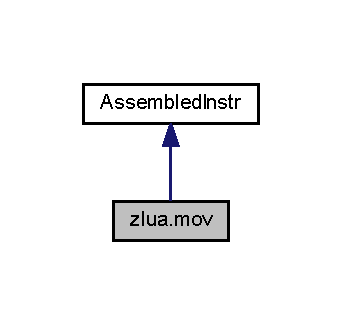
\includegraphics[width=164pt]{classzlua_1_1mov__inherit__graph}
\end{center}
\end{figure}


Collaboration diagram for zlua.\+mov\+:
\nopagebreak
\begin{figure}[H]
\begin{center}
\leavevmode
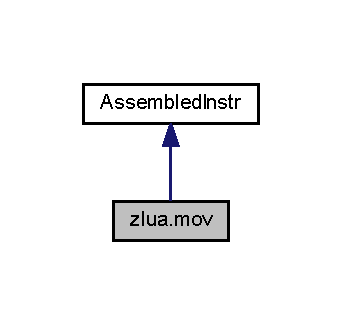
\includegraphics[width=164pt]{classzlua_1_1mov__coll__graph}
\end{center}
\end{figure}
\subsection*{Public Member Functions}
\begin{DoxyCompactItemize}
\item 
override void \mbox{\hyperlink{classzlua_1_1mov_a729d173bb798f765ed20aabcfaf2f63c}{execute}} (\mbox{\hyperlink{classzlua_1_1lua___thread}{lua\+\_\+\+Thread}} thread)
\begin{DoxyCompactList}\small\item\em differ from py ver\+: C\# dont have meta programming, so must use polymorphic to implement visitor pattern and cause execution is in Instr env (I\+OC) \end{DoxyCompactList}\item 
\mbox{\Hypertarget{classzlua_1_1mov_aa3978dc1bdda57d553a9d99a0104b336}\label{classzlua_1_1mov_aa3978dc1bdda57d553a9d99a0104b336}} 
override string {\bfseries To\+String} ()
\item 
\mbox{\Hypertarget{classzlua_1_1mov_a6a5c59944ace654350aa1a97486a01d5}\label{classzlua_1_1mov_a6a5c59944ace654350aa1a97486a01d5}} 
{\bfseries mov} (string var\+\_\+name)
\end{DoxyCompactItemize}
\subsection*{Additional Inherited Members}


\subsection{Member Function Documentation}
\mbox{\Hypertarget{classzlua_1_1mov_a729d173bb798f765ed20aabcfaf2f63c}\label{classzlua_1_1mov_a729d173bb798f765ed20aabcfaf2f63c}} 
\index{zlua\+::mov@{zlua\+::mov}!execute@{execute}}
\index{execute@{execute}!zlua\+::mov@{zlua\+::mov}}
\subsubsection{\texorpdfstring{execute()}{execute()}}
{\footnotesize\ttfamily override void zlua.\+mov.\+execute (\begin{DoxyParamCaption}\item[{\mbox{\hyperlink{classzlua_1_1lua___thread}{lua\+\_\+\+Thread}}}]{thread }\end{DoxyParamCaption})\hspace{0.3cm}{\ttfamily [virtual]}}



differ from py ver\+: C\# dont have meta programming, so must use polymorphic to implement visitor pattern and cause execution is in Instr env (I\+OC) 


\begin{DoxyParams}{Parameters}
{\em thread} & \\
\hline
\end{DoxyParams}


Implements \mbox{\hyperlink{classzlua_1_1_assembled_instr_a44e081c4565b90b75e4a67b8dd418feb}{zlua.\+Assembled\+Instr}}.



The documentation for this class was generated from the following file\+:\begin{DoxyCompactItemize}
\item 
zlua/I\+S\+A.\+cs\end{DoxyCompactItemize}

\hypertarget{classzlua_1_1mul}{}\section{zlua.\+mul Class Reference}
\label{classzlua_1_1mul}\index{zlua.\+mul@{zlua.\+mul}}


Inheritance diagram for zlua.\+mul\+:
\nopagebreak
\begin{figure}[H]
\begin{center}
\leavevmode
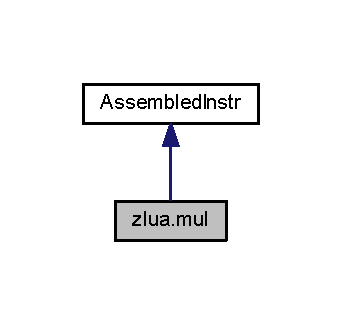
\includegraphics[width=164pt]{classzlua_1_1mul__inherit__graph}
\end{center}
\end{figure}


Collaboration diagram for zlua.\+mul\+:
\nopagebreak
\begin{figure}[H]
\begin{center}
\leavevmode
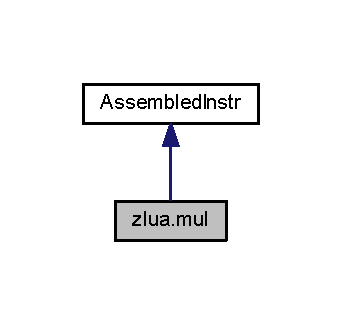
\includegraphics[width=164pt]{classzlua_1_1mul__coll__graph}
\end{center}
\end{figure}
\subsection*{Public Member Functions}
\begin{DoxyCompactItemize}
\item 
override void \mbox{\hyperlink{classzlua_1_1mul_a22002ab020aaabcf37eddae16b6ba10a}{execute}} (\mbox{\hyperlink{classzlua_1_1lua___thread}{lua\+\_\+\+Thread}} thread)
\begin{DoxyCompactList}\small\item\em differ from py ver\+: C\# dont have meta programming, so must use polymorphic to implement visitor pattern and cause execution is in Instr env (I\+OC) \end{DoxyCompactList}\item 
\mbox{\Hypertarget{classzlua_1_1mul_a17eb2965f4186881cb5ad9f0e8981307}\label{classzlua_1_1mul_a17eb2965f4186881cb5ad9f0e8981307}} 
override string {\bfseries To\+String} ()
\end{DoxyCompactItemize}
\subsection*{Additional Inherited Members}


\subsection{Member Function Documentation}
\mbox{\Hypertarget{classzlua_1_1mul_a22002ab020aaabcf37eddae16b6ba10a}\label{classzlua_1_1mul_a22002ab020aaabcf37eddae16b6ba10a}} 
\index{zlua\+::mul@{zlua\+::mul}!execute@{execute}}
\index{execute@{execute}!zlua\+::mul@{zlua\+::mul}}
\subsubsection{\texorpdfstring{execute()}{execute()}}
{\footnotesize\ttfamily override void zlua.\+mul.\+execute (\begin{DoxyParamCaption}\item[{\mbox{\hyperlink{classzlua_1_1lua___thread}{lua\+\_\+\+Thread}}}]{thread }\end{DoxyParamCaption})\hspace{0.3cm}{\ttfamily [virtual]}}



differ from py ver\+: C\# dont have meta programming, so must use polymorphic to implement visitor pattern and cause execution is in Instr env (I\+OC) 


\begin{DoxyParams}{Parameters}
{\em thread} & \\
\hline
\end{DoxyParams}


Implements \mbox{\hyperlink{classzlua_1_1_assembled_instr_a44e081c4565b90b75e4a67b8dd418feb}{zlua.\+Assembled\+Instr}}.



The documentation for this class was generated from the following file\+:\begin{DoxyCompactItemize}
\item 
zlua/I\+S\+A.\+cs\end{DoxyCompactItemize}

\hypertarget{classzlua_1_1pop}{}\section{zlua.\+pop Class Reference}
\label{classzlua_1_1pop}\index{zlua.\+pop@{zlua.\+pop}}


Inheritance diagram for zlua.\+pop\+:
\nopagebreak
\begin{figure}[H]
\begin{center}
\leavevmode
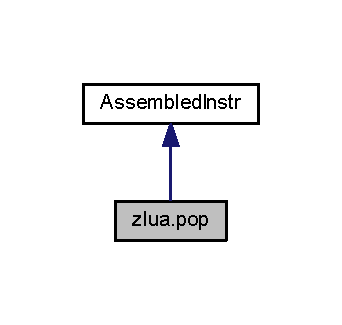
\includegraphics[width=164pt]{classzlua_1_1pop__inherit__graph}
\end{center}
\end{figure}


Collaboration diagram for zlua.\+pop\+:
\nopagebreak
\begin{figure}[H]
\begin{center}
\leavevmode
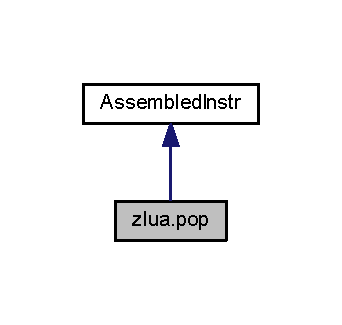
\includegraphics[width=164pt]{classzlua_1_1pop__coll__graph}
\end{center}
\end{figure}
\subsection*{Public Member Functions}
\begin{DoxyCompactItemize}
\item 
override void \mbox{\hyperlink{classzlua_1_1pop_a72cea959966aec69448d61be5bfc322c}{execute}} (\mbox{\hyperlink{classzlua_1_1lua___thread}{lua\+\_\+\+Thread}} thread)
\begin{DoxyCompactList}\small\item\em differ from py ver\+: C\# dont have meta programming, so must use polymorphic to implement visitor pattern and cause execution is in Instr env (I\+OC) \end{DoxyCompactList}\item 
\mbox{\Hypertarget{classzlua_1_1pop_ae497911a38afede3ce5c680583fd7a37}\label{classzlua_1_1pop_ae497911a38afede3ce5c680583fd7a37}} 
override string {\bfseries To\+String} ()
\end{DoxyCompactItemize}
\subsection*{Additional Inherited Members}


\subsection{Member Function Documentation}
\mbox{\Hypertarget{classzlua_1_1pop_a72cea959966aec69448d61be5bfc322c}\label{classzlua_1_1pop_a72cea959966aec69448d61be5bfc322c}} 
\index{zlua\+::pop@{zlua\+::pop}!execute@{execute}}
\index{execute@{execute}!zlua\+::pop@{zlua\+::pop}}
\subsubsection{\texorpdfstring{execute()}{execute()}}
{\footnotesize\ttfamily override void zlua.\+pop.\+execute (\begin{DoxyParamCaption}\item[{\mbox{\hyperlink{classzlua_1_1lua___thread}{lua\+\_\+\+Thread}}}]{thread }\end{DoxyParamCaption})\hspace{0.3cm}{\ttfamily [virtual]}}



differ from py ver\+: C\# dont have meta programming, so must use polymorphic to implement visitor pattern and cause execution is in Instr env (I\+OC) 


\begin{DoxyParams}{Parameters}
{\em thread} & \\
\hline
\end{DoxyParams}


Implements \mbox{\hyperlink{classzlua_1_1_assembled_instr_a44e081c4565b90b75e4a67b8dd418feb}{zlua.\+Assembled\+Instr}}.



The documentation for this class was generated from the following file\+:\begin{DoxyCompactItemize}
\item 
zlua/I\+S\+A.\+cs\end{DoxyCompactItemize}

\hypertarget{classzlua_1_1_program}{}\section{zlua.\+Program Class Reference}
\label{classzlua_1_1_program}\index{zlua.\+Program@{zlua.\+Program}}
\subsection*{Static Public Member Functions}
\begin{DoxyCompactItemize}
\item 
\mbox{\Hypertarget{classzlua_1_1_program_a432b86f3ddeb20105ae96a48414194ff}\label{classzlua_1_1_program_a432b86f3ddeb20105ae96a48414194ff}} 
static void {\bfseries Main} (string\mbox{[}$\,$\mbox{]} args)
\end{DoxyCompactItemize}


The documentation for this class was generated from the following file\+:\begin{DoxyCompactItemize}
\item 
zlua/Program.\+cs\end{DoxyCompactItemize}

\hypertarget{classzlua_1_1push}{}\section{zlua.\+push Class Reference}
\label{classzlua_1_1push}\index{zlua.\+push@{zlua.\+push}}


Inheritance diagram for zlua.\+push\+:
\nopagebreak
\begin{figure}[H]
\begin{center}
\leavevmode
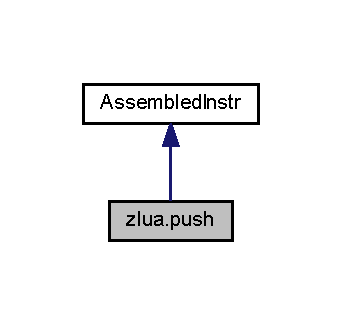
\includegraphics[width=164pt]{classzlua_1_1push__inherit__graph}
\end{center}
\end{figure}


Collaboration diagram for zlua.\+push\+:
\nopagebreak
\begin{figure}[H]
\begin{center}
\leavevmode
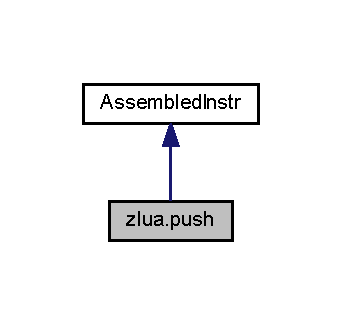
\includegraphics[width=164pt]{classzlua_1_1push__coll__graph}
\end{center}
\end{figure}
\subsection*{Public Member Functions}
\begin{DoxyCompactItemize}
\item 
\mbox{\Hypertarget{classzlua_1_1push_a5b00663f4af8797023a2f9b3ad4341a2}\label{classzlua_1_1push_a5b00663f4af8797023a2f9b3ad4341a2}} 
{\bfseries push} (\mbox{\hyperlink{classzlua_1_1lua___t_value}{lua\+\_\+\+T\+Value}} item)
\item 
override void \mbox{\hyperlink{classzlua_1_1push_ab3284599ae65d600d21622bd407405e8}{execute}} (\mbox{\hyperlink{classzlua_1_1lua___thread}{lua\+\_\+\+Thread}} thread)
\begin{DoxyCompactList}\small\item\em differ from py ver\+: C\# dont have meta programming, so must use polymorphic to implement visitor pattern and cause execution is in Instr env (I\+OC) \end{DoxyCompactList}\item 
\mbox{\Hypertarget{classzlua_1_1push_ab785fcb2a7de273f23f66a2ed04d4fff}\label{classzlua_1_1push_ab785fcb2a7de273f23f66a2ed04d4fff}} 
override string {\bfseries To\+String} ()
\end{DoxyCompactItemize}
\subsection*{Additional Inherited Members}


\subsection{Member Function Documentation}
\mbox{\Hypertarget{classzlua_1_1push_ab3284599ae65d600d21622bd407405e8}\label{classzlua_1_1push_ab3284599ae65d600d21622bd407405e8}} 
\index{zlua\+::push@{zlua\+::push}!execute@{execute}}
\index{execute@{execute}!zlua\+::push@{zlua\+::push}}
\subsubsection{\texorpdfstring{execute()}{execute()}}
{\footnotesize\ttfamily override void zlua.\+push.\+execute (\begin{DoxyParamCaption}\item[{\mbox{\hyperlink{classzlua_1_1lua___thread}{lua\+\_\+\+Thread}}}]{thread }\end{DoxyParamCaption})\hspace{0.3cm}{\ttfamily [virtual]}}



differ from py ver\+: C\# dont have meta programming, so must use polymorphic to implement visitor pattern and cause execution is in Instr env (I\+OC) 


\begin{DoxyParams}{Parameters}
{\em thread} & \\
\hline
\end{DoxyParams}


Implements \mbox{\hyperlink{classzlua_1_1_assembled_instr_a44e081c4565b90b75e4a67b8dd418feb}{zlua.\+Assembled\+Instr}}.



The documentation for this class was generated from the following file\+:\begin{DoxyCompactItemize}
\item 
zlua/I\+S\+A.\+cs\end{DoxyCompactItemize}

\hypertarget{classzlua_1_1push__var}{}\section{zlua.\+push\+\_\+var Class Reference}
\label{classzlua_1_1push__var}\index{zlua.\+push\+\_\+var@{zlua.\+push\+\_\+var}}


Inheritance diagram for zlua.\+push\+\_\+var\+:
\nopagebreak
\begin{figure}[H]
\begin{center}
\leavevmode
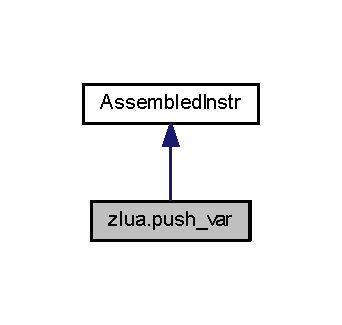
\includegraphics[width=164pt]{classzlua_1_1push__var__inherit__graph}
\end{center}
\end{figure}


Collaboration diagram for zlua.\+push\+\_\+var\+:
\nopagebreak
\begin{figure}[H]
\begin{center}
\leavevmode
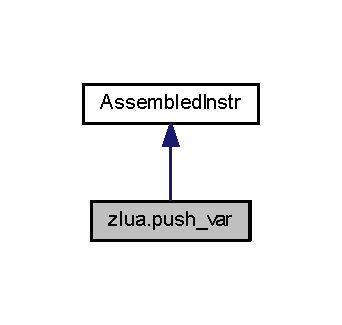
\includegraphics[width=164pt]{classzlua_1_1push__var__coll__graph}
\end{center}
\end{figure}
\subsection*{Public Member Functions}
\begin{DoxyCompactItemize}
\item 
\mbox{\Hypertarget{classzlua_1_1push__var_ac064959492641889ff53e2eac66e904c}\label{classzlua_1_1push__var_ac064959492641889ff53e2eac66e904c}} 
{\bfseries push\+\_\+var} (string var\+\_\+name)
\item 
override void \mbox{\hyperlink{classzlua_1_1push__var_a854bc287123c636f0c3d86735938879f}{execute}} (\mbox{\hyperlink{classzlua_1_1lua___thread}{lua\+\_\+\+Thread}} thread)
\begin{DoxyCompactList}\small\item\em differ from py ver\+: C\# dont have meta programming, so must use polymorphic to implement visitor pattern and cause execution is in Instr env (I\+OC) \end{DoxyCompactList}\item 
\mbox{\Hypertarget{classzlua_1_1push__var_afae2c8d51a5d2bbcc678103030185766}\label{classzlua_1_1push__var_afae2c8d51a5d2bbcc678103030185766}} 
override string {\bfseries To\+String} ()
\end{DoxyCompactItemize}
\subsection*{Additional Inherited Members}


\subsection{Member Function Documentation}
\mbox{\Hypertarget{classzlua_1_1push__var_a854bc287123c636f0c3d86735938879f}\label{classzlua_1_1push__var_a854bc287123c636f0c3d86735938879f}} 
\index{zlua\+::push\+\_\+var@{zlua\+::push\+\_\+var}!execute@{execute}}
\index{execute@{execute}!zlua\+::push\+\_\+var@{zlua\+::push\+\_\+var}}
\subsubsection{\texorpdfstring{execute()}{execute()}}
{\footnotesize\ttfamily override void zlua.\+push\+\_\+var.\+execute (\begin{DoxyParamCaption}\item[{\mbox{\hyperlink{classzlua_1_1lua___thread}{lua\+\_\+\+Thread}}}]{thread }\end{DoxyParamCaption})\hspace{0.3cm}{\ttfamily [virtual]}}



differ from py ver\+: C\# dont have meta programming, so must use polymorphic to implement visitor pattern and cause execution is in Instr env (I\+OC) 


\begin{DoxyParams}{Parameters}
{\em thread} & \\
\hline
\end{DoxyParams}


Implements \mbox{\hyperlink{classzlua_1_1_assembled_instr_a44e081c4565b90b75e4a67b8dd418feb}{zlua.\+Assembled\+Instr}}.



The documentation for this class was generated from the following file\+:\begin{DoxyCompactItemize}
\item 
zlua/I\+S\+A.\+cs\end{DoxyCompactItemize}

\hypertarget{classzlua_1_1ret}{}\section{zlua.\+ret Class Reference}
\label{classzlua_1_1ret}\index{zlua.\+ret@{zlua.\+ret}}


Inheritance diagram for zlua.\+ret\+:
\nopagebreak
\begin{figure}[H]
\begin{center}
\leavevmode
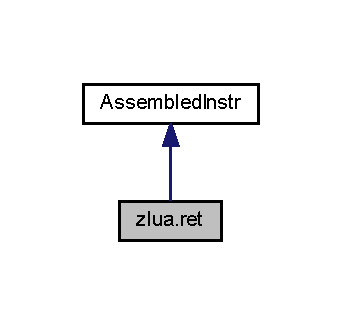
\includegraphics[width=164pt]{classzlua_1_1ret__inherit__graph}
\end{center}
\end{figure}


Collaboration diagram for zlua.\+ret\+:
\nopagebreak
\begin{figure}[H]
\begin{center}
\leavevmode
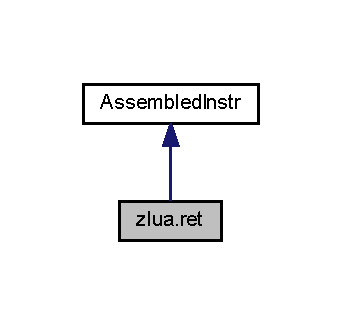
\includegraphics[width=164pt]{classzlua_1_1ret__coll__graph}
\end{center}
\end{figure}
\subsection*{Public Member Functions}
\begin{DoxyCompactItemize}
\item 
override void \mbox{\hyperlink{classzlua_1_1ret_a0c334b18dbe8e21c26aa785269b29253}{execute}} (\mbox{\hyperlink{classzlua_1_1lua___thread}{lua\+\_\+\+Thread}} thread)
\begin{DoxyCompactList}\small\item\em differ from py ver\+: C\# dont have meta programming, so must use polymorphic to implement visitor pattern and cause execution is in Instr env (I\+OC) \end{DoxyCompactList}\item 
\mbox{\Hypertarget{classzlua_1_1ret_a7e5681dd57149b9d11f503e980a5acef}\label{classzlua_1_1ret_a7e5681dd57149b9d11f503e980a5acef}} 
override string {\bfseries To\+String} ()
\end{DoxyCompactItemize}
\subsection*{Additional Inherited Members}


\subsection{Member Function Documentation}
\mbox{\Hypertarget{classzlua_1_1ret_a0c334b18dbe8e21c26aa785269b29253}\label{classzlua_1_1ret_a0c334b18dbe8e21c26aa785269b29253}} 
\index{zlua\+::ret@{zlua\+::ret}!execute@{execute}}
\index{execute@{execute}!zlua\+::ret@{zlua\+::ret}}
\subsubsection{\texorpdfstring{execute()}{execute()}}
{\footnotesize\ttfamily override void zlua.\+ret.\+execute (\begin{DoxyParamCaption}\item[{\mbox{\hyperlink{classzlua_1_1lua___thread}{lua\+\_\+\+Thread}}}]{thread }\end{DoxyParamCaption})\hspace{0.3cm}{\ttfamily [virtual]}}



differ from py ver\+: C\# dont have meta programming, so must use polymorphic to implement visitor pattern and cause execution is in Instr env (I\+OC) 


\begin{DoxyParams}{Parameters}
{\em thread} & \\
\hline
\end{DoxyParams}


Implements \mbox{\hyperlink{classzlua_1_1_assembled_instr_a44e081c4565b90b75e4a67b8dd418feb}{zlua.\+Assembled\+Instr}}.



The documentation for this class was generated from the following file\+:\begin{DoxyCompactItemize}
\item 
zlua/I\+S\+A.\+cs\end{DoxyCompactItemize}

\hypertarget{classzlua_1_1_runtime_func}{}\section{zlua.\+Runtime\+Func Class Reference}
\label{classzlua_1_1_runtime_func}\index{zlua.\+Runtime\+Func@{zlua.\+Runtime\+Func}}


\char`\"{}\+Clousure\char`\"{} in lua.\+c  




Inheritance diagram for zlua.\+Runtime\+Func\+:
\nopagebreak
\begin{figure}[H]
\begin{center}
\leavevmode
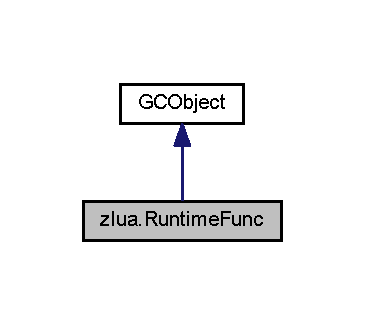
\includegraphics[width=175pt]{classzlua_1_1_runtime_func__inherit__graph}
\end{center}
\end{figure}


Collaboration diagram for zlua.\+Runtime\+Func\+:
\nopagebreak
\begin{figure}[H]
\begin{center}
\leavevmode
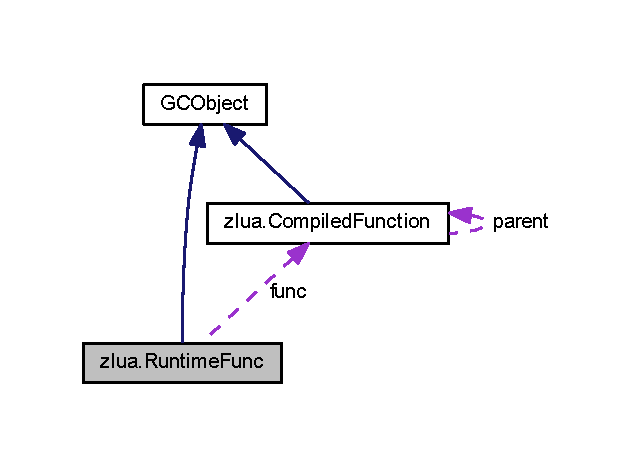
\includegraphics[width=305pt]{classzlua_1_1_runtime_func__coll__graph}
\end{center}
\end{figure}
\subsection*{Public Member Functions}
\begin{DoxyCompactItemize}
\item 
\mbox{\Hypertarget{classzlua_1_1_runtime_func_aeea097d2d35cfc06c0a03cb2164286ca}\label{classzlua_1_1_runtime_func_aeea097d2d35cfc06c0a03cb2164286ca}} 
{\bfseries Runtime\+Func} (\mbox{\hyperlink{classzlua_1_1_compiled_function}{Compiled\+Function}} func)
\end{DoxyCompactItemize}
\subsection*{Public Attributes}
\begin{DoxyCompactItemize}
\item 
\mbox{\Hypertarget{classzlua_1_1_runtime_func_a753d0bf3e22f4ddc65048bdc65b2469c}\label{classzlua_1_1_runtime_func_a753d0bf3e22f4ddc65048bdc65b2469c}} 
\mbox{\hyperlink{classzlua_1_1_compiled_function}{Compiled\+Function}} {\bfseries func}
\item 
\mbox{\Hypertarget{classzlua_1_1_runtime_func_a99d3029f09035ff1ab70e717ad1022f8}\label{classzlua_1_1_runtime_func_a99d3029f09035ff1ab70e717ad1022f8}} 
int {\bfseries ret\+\_\+addr}
\item 
\mbox{\Hypertarget{classzlua_1_1_runtime_func_a154f0ae1f0b750a133a6db5ea5d564d7}\label{classzlua_1_1_runtime_func_a154f0ae1f0b750a133a6db5ea5d564d7}} 
Dictionary$<$ string, \mbox{\hyperlink{classzlua_1_1lua___t_value}{lua\+\_\+\+T\+Value}} $>$ {\bfseries local\+\_\+data} = new Dictionary$<$string, \mbox{\hyperlink{classzlua_1_1lua___t_value}{lua\+\_\+\+T\+Value}}$>$()
\item 
\mbox{\Hypertarget{classzlua_1_1_runtime_func_a995a6f394890d8c97135f74f8c90c65c}\label{classzlua_1_1_runtime_func_a995a6f394890d8c97135f74f8c90c65c}} 
Stack$<$ \mbox{\hyperlink{classzlua_1_1lua___t_value}{lua\+\_\+\+T\+Value}} $>$ {\bfseries stack} = new Stack$<$\mbox{\hyperlink{classzlua_1_1lua___t_value}{lua\+\_\+\+T\+Value}}$>$()
\end{DoxyCompactItemize}
\subsection*{Additional Inherited Members}


\subsection{Detailed Description}
\char`\"{}\+Clousure\char`\"{} in lua.\+c 



The documentation for this class was generated from the following file\+:\begin{DoxyCompactItemize}
\item 
zlua/lobject.\+cs\end{DoxyCompactItemize}

\hypertarget{classzlua_1_1_t_string}{}\section{zlua.\+T\+String Class Reference}
\label{classzlua_1_1_t_string}\index{zlua.\+T\+String@{zlua.\+T\+String}}


the string type of lua, just warpper of C\# string  




Inheritance diagram for zlua.\+T\+String\+:
\nopagebreak
\begin{figure}[H]
\begin{center}
\leavevmode
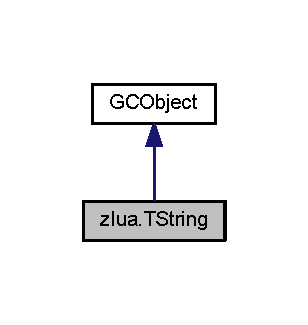
\includegraphics[width=148pt]{classzlua_1_1_t_string__inherit__graph}
\end{center}
\end{figure}


Collaboration diagram for zlua.\+T\+String\+:
\nopagebreak
\begin{figure}[H]
\begin{center}
\leavevmode
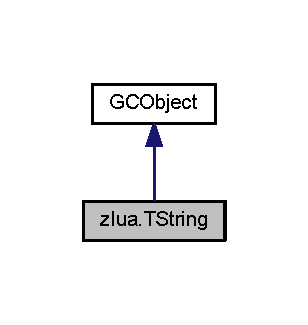
\includegraphics[width=148pt]{classzlua_1_1_t_string__coll__graph}
\end{center}
\end{figure}
\subsection*{Public Member Functions}
\begin{DoxyCompactItemize}
\item 
\mbox{\Hypertarget{classzlua_1_1_t_string_aa8a0265433abc7f66b052c192510e5e6}\label{classzlua_1_1_t_string_aa8a0265433abc7f66b052c192510e5e6}} 
{\bfseries T\+String} (string str)
\item 
\mbox{\Hypertarget{classzlua_1_1_t_string_a1ae6d043e64e48ebd9ad4ac6b118edf3}\label{classzlua_1_1_t_string_a1ae6d043e64e48ebd9ad4ac6b118edf3}} 
override string {\bfseries To\+String} ()
\end{DoxyCompactItemize}
\subsection*{Public Attributes}
\begin{DoxyCompactItemize}
\item 
\mbox{\Hypertarget{classzlua_1_1_t_string_a35ab6c458880b6b8da5db37675809357}\label{classzlua_1_1_t_string_a35ab6c458880b6b8da5db37675809357}} 
string {\bfseries str}
\end{DoxyCompactItemize}
\subsection*{Additional Inherited Members}


\subsection{Detailed Description}
the string type of lua, just warpper of C\# string 



The documentation for this class was generated from the following file\+:\begin{DoxyCompactItemize}
\item 
zlua/lobject.\+cs\end{DoxyCompactItemize}

\hypertarget{classzlua_1_1_value}{}\section{zlua.\+Value Class Reference}
\label{classzlua_1_1_value}\index{zlua.\+Value@{zlua.\+Value}}


(C\# simulated) union of all lua values how it simulate union?\+: use extra fields size\+: 8+8+4=20\+Byte differ from clua\+: light userdata is removed because C\# use GC  


\subsection*{Properties}
\begin{DoxyCompactItemize}
\item 
\mbox{\hyperlink{classzlua_1_1_g_c_object}{G\+C\+Object}} \mbox{\hyperlink{classzlua_1_1_value_af997ede3cb8de1aceb31d342a3f878bb}{gcobject}}\hspace{0.3cm}{\ttfamily  \mbox{[}get, set\mbox{]}}
\begin{DoxyCompactList}\small\item\em the GC collectable object \end{DoxyCompactList}\item 
lua\+\_\+\+Number \mbox{\hyperlink{classzlua_1_1_value_a2e93be2270276b85ddbbe0eb6e1cf447}{n}}\hspace{0.3cm}{\ttfamily  \mbox{[}get, set\mbox{]}}
\begin{DoxyCompactList}\small\item\em the number type of lua \end{DoxyCompactList}\item 
int \mbox{\hyperlink{classzlua_1_1_value_a310972c4cacdce5ad26c822d4837591d}{i}}\hspace{0.3cm}{\ttfamily  \mbox{[}get, set\mbox{]}}
\begin{DoxyCompactList}\small\item\em the int type of lua \end{DoxyCompactList}\item 
\mbox{\Hypertarget{classzlua_1_1_value_a4bfc8554ad810a169d2eda2e6f0f234d}\label{classzlua_1_1_value_a4bfc8554ad810a169d2eda2e6f0f234d}} 
bool {\bfseries b}\hspace{0.3cm}{\ttfamily  \mbox{[}get, set\mbox{]}}
\end{DoxyCompactItemize}


\subsection{Detailed Description}
(C\# simulated) union of all lua values how it simulate union?\+: use extra fields size\+: 8+8+4=20\+Byte differ from clua\+: light userdata is removed because C\# use GC 



\subsection{Property Documentation}
\mbox{\Hypertarget{classzlua_1_1_value_af997ede3cb8de1aceb31d342a3f878bb}\label{classzlua_1_1_value_af997ede3cb8de1aceb31d342a3f878bb}} 
\index{zlua\+::\+Value@{zlua\+::\+Value}!gcobject@{gcobject}}
\index{gcobject@{gcobject}!zlua\+::\+Value@{zlua\+::\+Value}}
\subsubsection{\texorpdfstring{gcobject}{gcobject}}
{\footnotesize\ttfamily \mbox{\hyperlink{classzlua_1_1_g_c_object}{G\+C\+Object}} zlua.\+Value.\+gcobject\hspace{0.3cm}{\ttfamily [get]}, {\ttfamily [set]}}



the GC collectable object 

\mbox{\Hypertarget{classzlua_1_1_value_a310972c4cacdce5ad26c822d4837591d}\label{classzlua_1_1_value_a310972c4cacdce5ad26c822d4837591d}} 
\index{zlua\+::\+Value@{zlua\+::\+Value}!i@{i}}
\index{i@{i}!zlua\+::\+Value@{zlua\+::\+Value}}
\subsubsection{\texorpdfstring{i}{i}}
{\footnotesize\ttfamily int zlua.\+Value.\+i\hspace{0.3cm}{\ttfamily [get]}, {\ttfamily [set]}}



the int type of lua 

\mbox{\Hypertarget{classzlua_1_1_value_a2e93be2270276b85ddbbe0eb6e1cf447}\label{classzlua_1_1_value_a2e93be2270276b85ddbbe0eb6e1cf447}} 
\index{zlua\+::\+Value@{zlua\+::\+Value}!n@{n}}
\index{n@{n}!zlua\+::\+Value@{zlua\+::\+Value}}
\subsubsection{\texorpdfstring{n}{n}}
{\footnotesize\ttfamily lua\+\_\+\+Number zlua.\+Value.\+n\hspace{0.3cm}{\ttfamily [get]}, {\ttfamily [set]}}



the number type of lua 



The documentation for this class was generated from the following file\+:\begin{DoxyCompactItemize}
\item 
zlua/lobject.\+cs\end{DoxyCompactItemize}

%--- End generated contents ---

% Index
\backmatter
\newpage
\phantomsection
\clearemptydoublepage
\addcontentsline{toc}{chapter}{Index}
\printindex

\end{document}
